\chapter{Lexical problem solving: Internet research}
\label{sec:9}

The first \isi{problem solving strategy} that will be analysed examines the instances in which the participants looked up words or phrases in the Internet. Hence, we will look at \isi{external resources}\footnote{Find details on internal vs. external resources in the next chapter}. This strategy is accordingly classified as a conscious problem solving strategy because the translators actively decide that they have difficulties with a certain text part and therefore consult an Internet-based resource to find help. The following sub-sections will first introduce the theme of lexical research, theoretical assumptions, and previous studies. Then, the focus will be on the evaluation of the translation process data of the experiments according to screen-recording, eyetracking and keylogging data.

\section{Lexical problem solving: Introduction}
\label{sec:9:1}

The use of \isi{dictionaries} and other \isi{translation aids} is a topic that has already been studied to some degree in empirical translation studies. This graspable and expressive part of the translation process can provide valuable insights to translation behaviour in general as well as differences between professionals, semi-professional, and laypersons.


In regard to general \isi{lexical research behaviour}, %\label{ref:ZOTEROITEMCSLCITATIONcitationIDlFClNSzPpropertiesformattedCitationrtfMuc0u252llerSpitzerWolferandKoplenig2015plainCitationMllerSpitzerWolferandKoplenig2015citationItemsid162urishttpzoteroorgusers1255332itemsJPIHJA38urihttpzoteroorgusers1255332itemsJPIHJA38itemDataid162typearticlejournaltitleObservingonlinedictionaryusersStudiesusingwiktionarylogfilescontainertitleInternationalJournalofLexicographypage126volume28issue1authorfamilyMllerSpitzergivenCarolinfamilyWolfergivenSaschafamilyKopleniggivenAlexanderissueddateparts2015schemahttpsgithubcomcitationstylelanguageschemarawmastercslcitationjsonRNDqfKpjkJKKt}
\citet{Muller-SpitzerEtAl2015} examine the log files from 2013 of the \ili{German} version of Wiktionary to observe the behaviour of the users. They find a relationship between corpus frequencies of the individual words and how often these words were looked up in the dictionary. Further, polysemantic words are looked up more often than monosemantic words. Social relevance additionally impacts the lookup rate.


%\label{ref:ZOTEROITEMCSLCITATIONcitationIDVvKVyLZupropertiesformattedCitationRisku1998plainCitationRisku1998citationItemsid81urishttpzoteroorgusers1255332items5AWQUSUMurihttpzoteroorgusers1255332items5AWQUSUMitemDataid81typebooktitleTranslatorischeKompetenzpublisherStauffenburgpublisherplaceTbingeneventplaceTbingenauthorfamilyRiskugivenHannaissueddateparts1998schemahttpsgithubcomcitationstylelanguageschemarawmastercslcitationjsonRND3SfHNlHlfP}
\citet[160--175]{Risku1998} points out that two \isi{sources of information integration} exist in the translation process: first, the existing knowledge and the reference material provided by the client and, second, research. Research comprises much more than only dictionaries and terminology lists. Often, translation also requires using encyclopedias, domain-specific books\slash texts, or parallel texts as well as asking other translators, experts in the domain, or the client concrete questions on contents of the text. Further, the way in which translators conduct research supposedly differs significantly between beginner and expert translators. Risku assumes that research strategies of expert translators are not universal and distinct, but flexible and problem-oriented. However, three general tendencies might be identifiable: Experts use research, draw on abstract problem representation, and adapt their research according to needs and the available time.


In a study with professional translators and foreign language teachers, the %\label{ref:ZOTEROITEMCSLCITATIONcitationIDzHjK2onWpropertiesformattedCitationPACTE2005plainCitationPACTE2005citationItemsid223urishttpzoteroorgusers1255332itemsJBVNW3TJurihttpzoteroorgusers1255332itemsJBVNW3TJitemDataid223typearticlejournaltitleInvestigatingtranslationcompetencecontainertitleMetajournaldestraducteurspage0609619volume50issue2authorfamilyPACTEgivenGrupissueddateparts2005schemahttpsgithubcomcitationstylelanguageschemarawmastercslcitationjsonRND3muKTxi5bx}
\citet{Pacte2005} group analyses the types of resources used in the translation process. They suggest two main sources: internal and external resources. \isi{Internal resources} describe the knowledge the translator already has, while \isi{external resources} consolidate all information gathering processes. However, it is not always one or the other type of resource that is used exclusively by the translator, but a combination of both resources is often used to generate a translation solution. These can be identified according to the actions the translators undertake during translation. While a total of 16 types of actions were identified in the exploratory test, five were selected to identify the resources: reading the source text, pauses longer than five seconds, provisional solutions, definitive solutions, and consultations. According to these actions, five sub-categories of resources used during translation were identified (cf. ibid.: 615-616):


\begin{itemize}
\item \isi{Simple internal support} – the translator only uses his\slash her knowledge;
\item \isi{Mainly internal support with additional external support} – translation aids are consulted, but do not directly help to find the final translation choice;
\item \isi{Balanced internal and external support} -- translation decisions are created with both resources taken into account;
\item \isi{Mainly external support with additional internal support} – complex consultation of external resources from which the solution is drawn;
\item \isi{Simple external support} – a bilingual dictionary is used to find the solution.
\end{itemize}

% \begin{itemize}

This schema was adapted in a few studies – as introduced in %\label{ref:ZOTEROITEMCSLCITATIONcitationIDFlocfaGGpropertiesformattedCitationAlvesandLipariniCampos2009plainCitationAlvesandLipariniCampos2009citationItemsid159urishttpzoteroorgusers1255332items55KBCPU8urihttpzoteroorgusers1255332items55KBCPU8itemDataid159typechaptertitleTranslationtechnologyintimeInvestigatingtheimpactoftranslationmemorysystemsandtimepressureontypesofinternalandexternalsupportcontainertitleBehindtheMindMethodsModelsandResultsinTranslationProcessResearchpublisherCopenhagenStudiesinLanguagepublisherplaceCopenhagenpage191218volume37eventplaceCopenhagenauthorfamilyAlvesgivenFabiofamilyLipariniCamposgivenTaniaeditorfamilyGpferichgivenSusannefamilyJakobsengivenArntLykkefamilyMeesgivenIngerMissueddateparts2009schemahttpsgithubcomcitationstylelanguageschemarawmastercslcitationjsonRNDJi55CFk1pM}
\citet{AlvesLipariniCampos2009} – according to %\label{ref:ZOTEROITEMCSLCITATIONcitationIDpzphHRhzpropertiesformattedCitationJakobsen2005plainCitationJakobsen2005citationItemsid112urishttpzoteroorgusers1255332itemsKXHSKQDEurihttpzoteroorgusers1255332itemsKXHSKQDEitemDataid112typechaptertitleInvestigatingexperttranslatorsprocessingknowledgecontainertitleKnowledgesystemsandtranslationcollectiontitleTextTranslationComputationalProcessingTTCPcollectionnumber7publisherMoutondeGruyterpublisherplaceBerlinNewYorkeventplaceBerlinNewYorkauthorfamilyJakobsengivenArntLykkeeditorfamilyDamgivenHelleVfamilyEngberggivenJanfamilyGerzymischArbogastgivenHeidrunissueddateparts2005schemahttpsgithubcomcitationstylelanguageschemarawmastercslcitationjsonRNDAFM5HaIVGM}
\citegen{Jakobsen2005} notion that pauses indicate either \isi{orientation} or \isi{revision} processes. As resources can only be used for either orientation or revision – when a translation is drafted, a (first) translation decision has been made during orientation, which can be assessed afterwards, but is not done during the drafting process – the following sub-categories were developed:
% \end{itemize}
\begin{itemize}
\item simple internal support for orientation (SISO) and for revision (SISR)
\item simple external support for orientation (SESO) and for revision (SESR)
\item dominant internal support for orientation (DISO) and for revision (DISR)
\item dominant external support for orientation (DESO) and for revision (DESR)
\end{itemize}



This part of the study at hand will concentrate on \isi{external support}, which may or may not be used combined with internal resources. I suggest that most external research is combined with internal knowledge, except if a problem is purely lexical. And even then, the translator has knowledge about how this word\slash phrase is syntactically and grammatically embedded in the text and knows the context. Hence, (s)he knows how to make a decision for one or the other lexical choice offered by a dictionary etc.

In his think-aloud study, %\label{ref:ZOTEROITEMCSLCITATIONcitationIDdoNdCKSEpropertiesformattedCitationKrings1986plainCitationKrings1986dontUpdatetruecitationItemsid1709urishttpzoteroorggroups3587itemsX92T2ZTGurihttpzoteroorggroups3587itemsX92T2ZTGitemDataid1709typebooktitleWasindenKpfenvonbersetzernvorgehtEineempirischeUntersuchungzurStrukturdesbersetzungsprozessesanfortgeschrittenenFranzsischlernernpublisherGunterNarrVerlagpublisherplaceTbingeneventplaceTbingennoteZuglBochumUnivDiss198586authorfamilyKringsgivenHansPeterissueddateparts1986schemahttpsgithubcomcitationstylelanguageschemarawmastercslcitationjsonRNDydOgz8C5sk}
\citet[128]{Krings1986} observes that the use of aids is directly linked to \isi{problem solving} and can be easily determined in think-aloud protocols. The translators used aids in over 60\% of all detected problems – when they translated from their mother tongue into the foreign language, the participants used bilingual dictionaries in 80\% of the units identified as problems. Monolingual dictionaries were mainly used to find more information on a \isi{translation unit} in the foreign language (cf. ibid.: 166). However, compared to bilingual dictionaries, monolingual dictionaries played a minor role – they were not used for the translation into the mother tongue – and other aids no role at all (cf. ibd.: 218)\footnote{The participants were asked to bring their own printed aids, which were mainly dictionaries.}. Furthermore, many comprehension problems – about 75\% – were solved (or were tried to be solved) with the use of aids, and if they did not use aids, it was mostly because the participants were convinced that the dictionary would not contain the required entry. In only six out of 113 instances, the participants arrived at a solution to a problem via inferences according to the think-aloud protocols. This does not mean that participants do not use inferring as a strategy, but they hardly use it without any additional aids (cf. ibid.: 221-222). Although the participants in Krings' study are neither translation students nor professional translators, the study reveals that research is a very important indicator of problems in translation.


In her empirical study on translation aids, %\label{ref:ZOTEROITEMCSLCITATIONcitationIDJGA6VrgIpropertiesformattedCitationNord2002plainCitationNord2002dontUpdatetruecitationItemsid18urishttpzoteroorgusers1255332items252Z7TJQurihttpzoteroorgusers1255332items252Z7TJQitemDataid18typebooktitleHilfsmittelbeimbersetzeneineempirischeStudiezumRechercheverhaltenprofessionellerbersetzercollectiontitleFASKPublikationendesFachbereichsAngewandteSprachundKulturwissenschaftderJohannesGutenbergUniversittMainzinGermersheimcollectionnumberBd32publisherLangpublisherplaceFrankfurtamMainNewYorknumberofpages286sourceLibraryofCongressISBNeventplaceFrankfurtamMainNewYorkISBN3631393318callnumberP3065N672002shortTitleHilfsmittelbeimbersetzenauthorfamilyNordgivenBrittaissueddateparts2002schemahttpsgithubcomcitationstylelanguageschemarawmastercslcitationjsonRND0qbJJVhPBI}
\citet{Nord2002} analyses \isi{translation aids for research}. She divides translation aids (or external aids) in general into 


\begin{itemize}
\item \isi{physical aids for translation}, like a desk or a chair;
\item \isi{administration aids}, e.g. software to generate invoices, data bases;
\item \isi{communication aids}, like a telephone or an e-mail client;
\item \isi{text production aids}, like pencil and paper or computer hard- and software;
\item and finally the aforementioned \isi{research aids} that help with the translation itself and to expand the knowledge of the translator. (cf. ibid.: 6)
\end{itemize}

Special translation tools like \isi{translation memory} systems combine both text production and research aids. %\label{ref:ZOTEROITEMCSLCITATIONcitationIDbFYMfwpupropertiesformattedCitationNord2002plainCitationNord2002dontUpdatetruecitationItemsid18urishttpzoteroorgusers1255332items252Z7TJQurihttpzoteroorgusers1255332items252Z7TJQitemDataid18typebooktitleHilfsmittelbeimbersetzeneineempirischeStudiezumRechercheverhaltenprofessionellerbersetzercollectiontitleFASKPublikationendesFachbereichsAngewandteSprachundKulturwissenschaftderJohannesGutenbergUniversittMainzinGermersheimcollectionnumberBd32publisherLangpublisherplaceFrankfurtamMainNewYorknumberofpages286sourceLibraryofCongressISBNeventplaceFrankfurtamMainNewYorkISBN3631393318callnumberP3065N672002shortTitleHilfsmittelbeimbersetzenauthorfamilyNordgivenBrittaissueddateparts2002schemahttpsgithubcomcitationstylelanguageschemarawmastercslcitationjsonRNDmamHafOwXa}
Nord explores definitions of parallel texts and dictionary typologies and gives a detailed overview of the state of the art systematic and critical dictionary research in translation studies as well as research on dictionary use. Concerning critical dictionary research in translation studies, she concludes that translation scholars agree that bilingual dictionaries are not suitable translation aids as they do not incorporate text factors, the translation situation and the involved cultures. However, Nord criticises that, on the one hand, scholars do not define their understanding of translations and translators and hence consider different concepts. On the other hand she criticises\footnote{I fully agree with this point of criticism.} that they only explore the topic theoretically and not empirically (cf. ibid: 64-65). Next, she introduces some empirical studies on translation aids and finds little agreement in these studies. However, she highlights five fairly common results (cf. ibid.: 92):


\begin{itemize}
\item Less experienced translators tend to use bilingual dictionaries, while more experienced translators use monolingual dictionaries and other aids.
\item Dictionaries are used to find or check equivalents or the meaning of lexical units, or to determine alternative translations.
\item Translators use a translation aid 1.1 to 2.9 times per problem or source text unit. Experienced translators use translation aids more often than less experienced translators.
\item Monolingual dictionaries contain 84\% of the requested information, bilingual dictionaries only 54--73\%.
\item The use of dictionaries hardly improves the quality of the translation (which is measured very differently in the studies), some mistakes only emerge from the use of a dictionary.
\end{itemize}

For her study, \citet[102--114]{Nord2002} approached 16 professional translators (three for the pre-study, 13 for the main study) and observed them in their usual work environment. Every participant translated texts from his\slash her own everyday workload. The participants were asked to think aloud. However, the sessions were not recorded with a recording device but manually logged by the experimenter. Six parameters were evaluated: frequency of use, cause of use, reason for use, research request, choice of aid, and consequences of use. She concludes (cf. ibid.: 214-223) that translators need research aids and they need them very often (on average 17 times per hour). Different reasons for using dictionaries were found: either the translator does not understand the source text unit, (s)he does not know how to express the source unit in the target text, (s)he wants to recheck the own translation idea, or because the translator does not know how to integrate the target unit into the target text. The participants mainly used aids for lexical problems; missing domain and cultural knowledge is almost never the reason for research. Generally, they know how to handle research aids and know exactly which aid to use for which purpose.



The results of Nord’s study (cf. ibid.: 227-247) culminated in a theoretical framework for a specific translation dictionary and implications for teaching the use of translation aids. Her dictionary framework should be realised as a database that includes information on text type conventions, meaning, equivalents, use, spelling, grammar, context, synonyms, and non-linguistic information.



In the last decades, the world wide web became very influential and changed the work environments in many jobs – translation is no exception. While translators conventionally used printed media like mono-, bi-, and multilingual dictionaries, encyclopedias, etc., these research media are being increasingly replaced by electronic aids, which can be used on the computer either on- or offline. It is argued though that electronic research tools, especially online tools, do not necessarily accelerate the translation process, because the sources of the information need to be validated and that the information you can access on the Internet may be more error prone (cf. e.~g. %\label{ref:ZOTEROITEMCSLCITATIONcitationIDVKXnWrxbpropertiesformattedCitationAlbrecht2013plainCitationAlbrecht2013citationItemsid252urishttpzoteroorgusers1255332itemsVWXA4H73urihttpzoteroorgusers1255332itemsVWXA4H73itemDataid252typebooktitlebersetzungundLinguistikcollectiontitleGrundlagenderbersetzungsforschungcollectionnumberBd2publisherNarrpublisherplaceTbingennumberofpages312edition2berarbAuflsourceGemeinsamerBibliotheksverbundISBNeventplaceTbingenISBN9783823367932languagegerauthorfamilyAlbrechtgivenJrnissueddateparts2013schemahttpsgithubcomcitationstylelanguageschemarawmastercslcitationjsonRNDs0OQuJqHsY}
\citealt{Albrecht2013}: 60). Nonetheless, the experimental setup of the study at hand did not provide any printed research aids, because it is easier to record and follow the research process with \isi{electronic aids}. It is impossible to provide all printed aids that might be helpful for the participants; if only a selection is presented, it cannot be assumed that these are the favourite dictionaries etc. of the participants, which creates an unfamiliar work environment; even if the participants had been contacted before the experiments and had been asked to name their favourite printed translation aids they used most often, it could not have been guaranteed that these would be enough to cope with all lexical translation problems in the texts. Another aspect is that certain kinds of research aids like encyclopedias are hard to provide in a printed version. Bringing their own dictionaries was ruled out as it would have been an extra burden for the participants, they might have forgotten to bring their dictionaries, the research behaviour would not have been comparable, and the participants were not supposed to know which domain to prepare. Furthermore, it is assumed that the participants are trained in and used to using electronic aids from their daily work routine – both students and professional translators. They know which sources and websites they can trust and know how to assess the presented information. They were free to use everything available on the Internet, offline tools were not provided. Further, the study at hand is part of the \isi{CRITT-TPR database} and the same texts were translated\slash (monolingually) post-edited in many different languages (see \sectref{sec:7:2}). Hence, allowing all participants to use the online sources they prefer makes the study comparable.



In other translation process research studies, online tools were the only provided search aids, too. %\label{ref:ZOTEROITEMCSLCITATIONcitationIDPBmsxxGApropertiesformattedCitationDaemsetal2016plainCitationDaemsetal2016citationItemsid139urishttpzoteroorgusers1255332itemsQ53HQ4XIurihttpzoteroorgusers1255332itemsQ53HQ4XIitemDataid139typechaptertitleTheEffectivenessofConsultingExternalResourcesDuringTranslationandPosteditingofGeneralTextTypescontainertitleNewDirectionsinEmpiricalTranslationProcessResearchpublisherSpringerpublisherplaceHeidelbergNewYorkaopage111133eventplaceHeidelbergNewYorkaoauthorfamilyDaemsgivenJokefamilyCarlgivenMichaelfamilyVandepittegivenSoniafamilyHartsuikergivenRobertfamilyMackengivenLieveeditorfamilyCarlgivenMichaelfamilyBangaloregivenSrinivasfamilySchaeffergivenMoritzissueddateparts2016schemahttpsgithubcomcitationstylelanguageschemarawmastercslcitationjsonRNDkrBy3zDHz5}
\citet{DaemsEtAl2016} present a study in which they aim to compare participants' use of external resources during TfS and PE and to figure out how these \isi{external resources} can be used for successful problem solving concerning quality and productivity. The texts were translated in \isi{CASMACAT}, an online translation and PE environment, and the research instances were recorded with \isi{\textit{Inputlog}}, a \isi{keylogging tool}. Ten participants who were all studying for their Master's degree in translation studies were asked to translate and post-edit four newspaper texts each. All participants had no experience in PE. In the analysis, %\label{ref:ZOTEROITEMCSLCITATIONcitationIDVtKhCn6cpropertiesformattedCitationDaemsetal2016plainCitationDaemsetal2016citationItemsid139urishttpzoteroorgusers1255332itemsQ53HQ4XIurihttpzoteroorgusers1255332itemsQ53HQ4XIitemDataid139typechaptertitleTheEffectivenessofConsultingExternalResourcesDuringTranslationandPosteditingofGeneralTextTypescontainertitleNewDirectionsinEmpiricalTranslationProcessResearchpublisherSpringerpublisherplaceHeidelbergNewYorkaopage111133eventplaceHeidelbergNewYorkaoauthorfamilyDaemsgivenJokefamilyCarlgivenMichaelfamilyVandepittegivenSoniafamilyHartsuikergivenRobertfamilyMackengivenLieveeditorfamilyCarlgivenMichaelfamilyBangaloregivenSrinivasfamilySchaeffergivenMoritzissueddateparts2016schemahttpsgithubcomcitationstylelanguageschemarawmastercslcitationjsonRNDc4Yxbmqt2q}
Daems et al. grouped the used \isi{online resources} into five main types, i.e. search engines, concordancers, dictionaries, encyclopedias, and others. Next, they analysed the time the participants spent in external resources and found that the participants spent significantly more time for research in TfS than in the PE task. However, there was no significant relation between the types of aid used for external research and the task (cf. ibid.: 120-121). In terms of productivity, the participants needed significantly more time for human translation and also spent more time on research in this task. Further, the more often external research aids were used, the longer the overall session became (cf. ibid.: 123). The final criterion they analysed was the influence of external research aids on the quality of the text. As quality is a trait that is hard to measure, they developed a schema that focuses on acceptability and adequacy. No significant difference for quality was found between TfS and PE. However, the more sources were used in PE, the worse the quality of the final target text became; while in contrast, the more sources were used in human translation, the better the quality became. They explain this finding with the lack of experience in PE (as the participants have already developed successful research skills for human translation) and the priming effects of the MT output (cf. ibid.: 123-127). When adequacy and acceptability are considered individual quality criteria, no significant differences were found between TfS and PE. A longer or more frequent use of dictionaries seems to increase the quality of adequacy, while extensive research in encyclopedias seems to reduce acceptability of quality\footnote{%\label{ref:ZOTEROITEMCSLCITATIONcitationIDtgpTaJW3propertiesformattedCitationDaemsetal2016plainCitationDaemsetal2016citationItemsid139urishttpzoteroorgusers1255332itemsQ53HQ4XIurihttpzoteroorgusers1255332itemsQ53HQ4XIitemDataid139typechaptertitleTheEffectivenessofConsultingExternalResourcesDuringTranslationandPosteditingofGeneralTextTypescontainertitleNewDirectionsinEmpiricalTranslationProcessResearchpublisherSpringerpublisherplaceHeidelbergNewYorkaopage111133eventplaceHeidelbergNewYorkaoauthorfamilyDaemsgivenJokefamilyCarlgivenMichaelfamilyVandepittegivenSoniafamilyHartsuikergivenRobertfamilyMackengivenLieveeditorfamilyCarlgivenMichaelfamilyBangaloregivenSrinivasfamilySchaeffergivenMoritzissueddateparts2016schemahttpsgithubcomcitationstylelanguageschemarawmastercslcitationjsonRNDY22GA6wz0B}
\citet[130]{DaemsEtAl2016} explicitly point out that this relationship might not be causal.} (cf. ibid.: 127-131). They conclude their study with the statement that “whereas search strategies during the translation process are more effective than those used when PE, PE is still faster than human translation without negatively affecting the final quality of the product.” (ibid.: 131). The following chapter will quantify the Internet search instances in a similar way. However, these will not be analysed with regard to the quality of the final texts, but will be regarded as a problem solving indicator. Hence, I will compare the \isi{lexical problem solving behaviour} expressed by Internet research between TfS and PE\slash MPE as well as between professionals and semi-professionals.


To understand the nature of the problems in the texts, we will approach them lexically on a word or phrase level and will look at broader units in the next chapter (\sectref{sec:10}) on syntactic problems. In the context of the lexical analysis, I consider a \isi{\textit{phrase}} a word unit that contains more than one word; these words, however, share meaning and could be considered a semantic unit. The main focus of the analysis will be on the differences between PE and TfS. However, the MPE task will be analysed as well, because we can assume that most of the participants – students and professionals – have little experience in MPE\footnote{We have to remember that only 1/3 (cf. \sectref{sec:8:1}) of the participants have PE experience.} and therefore cannot draw on much task knowledge. Accordingly, the analysis will focus on the differences related to translation experience. The participants are separated into professional and semi-professional translators so that both groups can be compared. However, the groups are in themselves not uniform, which applies especially to the professional group – while one participant had only half a year of professional experience, another had 20 years experience. To get a more in-depth picture of the influence of experience, an \isi{\textit{experience coefficient}} will be used as well (see details in \sectref{sec:8:1}). It consists of the years of translation training plus two times the years of professional experience. Therefore, for example, a participant who spent five years studying translation and has 4.5 years of professional experience achieves a coefficient of 14.

Due to \isi{technical problems}, some of the sessions could not be replayed in Tobii Studio and accordingly the Internet search instances could not be observed. Although at least one session could not be replayed for every task, the total number of all sessions per tasks is almost equal and there is not a lot variation in the number of sessions per tasks. In the following table, the number of experiments that could be observed is listed (24 sessions should have been recorded per task):

\begin{table}
\begin{tabular}{lrrr}
\lsptoprule
 Task & Professionals & Students & Total\\
 \midrule 
 MPE & 20 & 23 & 43\\
 PE & 19 & 23 & 42\\
 TfS & 21 & 21 & 42\\
\lspbottomrule
\end{tabular}
%%please move \begin{table} just above \begin{tabular
\caption{Number of session recorded}
\label{tab:9:1}
\end{table}

\section{Lexical problem solving: screen recording data}
\label{sec:9:2}

This sub-chapter discuses the \isi{screen recording data} with regard to the \isi{Internet research} conducted by the participants. Screen recordings of the sessions are a useful method to protocol the use of research aids, which was traditionally done manually either by the experimenter or by the user him\slash herself, or via think-aloud protocols (cf. %\label{ref:ZOTEROITEMCSLCITATIONcitationIDoUSoYCdhpropertiesformattedCitationNord2002plainCitationNord2002dontUpdatetruecitationItemsid18urishttpzoteroorgusers1255332items252Z7TJQurihttpzoteroorgusers1255332items252Z7TJQitemDataid18typebooktitleHilfsmittelbeimbersetzeneineempirischeStudiezumRechercheverhaltenprofessionellerbersetzercollectiontitleFASKPublikationendesFachbereichsAngewandteSprachundKulturwissenschaftderJohannesGutenbergUniversittMainzinGermersheimcollectionnumberBd32publisherLangpublisherplaceFrankfurtamMainNewYorknumberofpages286sourceLibraryofCongressISBNeventplaceFrankfurtamMainNewYorkISBN3631393318callnumberP3065N672002shortTitleHilfsmittelbeimbersetzenauthorfamilyNordgivenBrittaissueddateparts2002schemahttpsgithubcomcitationstylelanguageschemarawmastercslcitationjsonRNDn3CQSvoNKT}
\citealt{Nord2002}: 99). The automatised capturing of the screen is less error prone compared to manual recordings and certainly complete if no technical difficulties occur that might leave us with no recording at all. The purpose of this analysis is to characterise the research behaviour of the participants before the keylogging and eyetracking data are analysed. First, the hypotheses for the screen recording data will be introduced and will be tested in the following sections.


\subsection{Introduction of hypotheses for lexical problem solving (screen recording data)}
\label{sec:9:2:1}

The overall hypothesis is that the different tasks show different \isi{search patterns}. The MT output might suggest translations for difficult or \isi{low-frequency words}\slash phrases that are acceptable and the translator does not need to do any research on the word\slash phrase. On the other hand, the MT might be lexically unacceptable in the context, e.g., inappropriate or incorrect collocations or wrong lexical choices, and might cause insecurity which, in turn, might make the translators research words which they may have not researched without the unacceptable \isi{MT output}. The Internet was used for context research, as well. Further, I assume that with a growing level of expertise, the translators show different patterns as well (find more details in \sectref{sec:6}), e.g., more research is done by less professional translators or less professional translators recheck their translation choices more often than more professional ones, because they are more insecure. Hence, the main hypothesis for external lexical research is:


\begin{itemize}
\item H: In the different tasks, the translators show different search patterns. The patterns also differ according to their expertise level.



H\textsubscript{0}: In the different tasks, the translators show the same search patterns. There is no difference between professionals and semi-professionals.
\end{itemize}




To disprove the null hypothesis, we will look at a number of subordinate hypotheses to cover different aspects of the topic, which are listed in the following. This is only done to give the reader an overview of covered topics. Detailed information on the object of investigation and the motivation for the individual hypotheses can be found in the respective section (indicated in brackets). These subordinate hypotheses are executed in the same order in the following chapters. Every hypothesis contains two sub-hypotheses – one concerning the different tasks, one concerning the difference between students and professionals – to keep the number manageable. This does not imply, however, that there is a compulsory relationship between task and professionalism.


\begin{itemize}
\item H\textsubscript{1}: The Internet is consulted more often in TfS than in the PE task. The Internet is consulted more often by students than by professionals.\footnote{We have to keep in mind that the PE instructions specifically stated that the participants should not “embark on time-consuming research” (see \sectref{sec:7:2}).} \textup{(\sectref{sec:9:2:2})}

H\textsubscript{01}: The Internet is consulted as often in TfS as in the PE task and students and professionals use it equally often.

\item H\textsubscript{2}: Fewer words\slash phrases are looked up in the PE tasks compared to TfS.\footnote{H\textsubscript{1} and H\textsubscript{2} are similar, but H\textsubscript{1} measures all research instance, without considering whether the same word\slash phrase was looked up more then once. H\textsubscript{2} considers only single words\slash phrases and not how often a word\slash phrase was researched.} However, when a word\slash phrase is looked up, the same word\slash phrase is looked up more often in PE. \textup{(\sectref{sec:9:2:3})}

H\textsubscript{02}: The amount of words\slash phrases looked up is equal in PE and TfS. Further, they are looked up equally often in both tasks.


\item H\textsubscript{3}: The Internet is not consulted in some sessions at all. This happens more often in the PE session than in the TfS session; and experts do not consult the Internet more often in the entire session than students. \textup{(\sectref{sec:9:2:4})}

H\textsubscript{03}: The Internet is not consulted in some sessions at all. This happens as often in the PE session as in the TfS, and both students and experts do not consult the Internet in the entire session to the same extent.


\item H\textsubscript{4}: The more complex a text, the more research is necessary. \textup{(\sectref{sec:9:2:5})}

H\textsubscript{04}: There is no connection between complexity level of a text and research effort.


\sloppy
\item H\textsubscript{5}: In both PE and TfS, the bilingual dictionary is the source that is used most often. This being said, bilingual dictionaries and other sources are distributed differently in both tasks. Students use bilingual dictionaries more often than professionals. (\sectref{sec:9:2:6})
\fussy 

H\textsubscript{05}: In both PE and TfS, the bilingual dictionary is not the source that is used most often and bilingual dictionaries and other sources are distributed equally in both tasks. Students and professionals use bilingual dictionaries equally often.


\item H\textsubscript{6.1}: Participants need more time for research per single word\slash phrase in PE than in TfS. Students need longer to find a translation than professionals if they research. \textup{(\sectref{sec:9:2:7})}

H\textsubscript{06.1}: Participants need as much time for research per single word\slash phrase in PE as in TfS. Students and professionals need equally long to find a translation if they research.

H\textsubscript{6.2}: Participants spend more time on research in TfS than in PE in the overall session. Students spend more time on research than professionals. \textup{(\sectref{sec:9:2:7})}

H\textsubscript{06.2}: Participants spend as much time on research in TfS as in PE in the overall session. Students and professionals spend the same time on research.


\item H\textsubscript{7}: Translators do most research in the drafting phase in TfS, while they do most research in the orientation and revision phase in PE. (\sectref{sec:9:2:8})

H\textsubscript{07}: Translators do research equally often in the same phases in TfS and PE.


\item H\textsubscript{8}: Students re-check their translations more often than professionals.\\ (\sectref{sec:9:2:9})

H\textsubscript{08}: Students and professionals re-check their translations equally often.
\end{itemize}


Both the grouping of the participants into professionals and students as well as the experience coefficient introduced in \sectref{sec:8:1} will be used to analyse the data. This is due to the simple reason that the experience coefficient is a new value that needs assessment for its general usability. Hence, both will be used throughout this book so that an assessment of the experience coefficient is possible at the end of this book.


\subsection{Number of research instances}
\label{sec:9:2:2}

\begin{quote}
H\textsubscript{1}: The Internet is consulted more often in TfS than in the PE task. The Internet is consulted more often by students than by professionals.
\end{quote}



As I assume that the MT output already solves some lexical problems, it is reasonable to predict that the translator has to consult the Internet more often in the TfS task than in PE, which was also already observed by %\label{ref:ZOTEROITEMCSLCITATIONcitationID7jyKd6hgpropertiesformattedCitationHansPKrings2001plainCitationHansPKrings2001citationItemsid228urishttpzoteroorgusers1255332items4D665XEKurihttpzoteroorgusers1255332items4D665XEKitemDataid228typebooktitleRepairingtextsempiricalinvestigationsofmachinetranslationposteditingprocessespublisherKentStateUniversityPresspublisherplaceKentOhionumberofpages635sourceLibraryofCongressISBNeventplaceKentOhioISBN9780873386715callnumberP309K75132001shortTitleRepairingtextslanguageengauthorfamilyKringsgivenHansPeditorfamilyKobygivenGeoffreySissueddateparts2001schemahttpsgithubcomcitationstylelanguageschemarawmastercslcitationjsonRNDqAg2bIyP9V}
\citet[318--320]{Krings2001}. Throughout all experiments, the Internet was consulted 685 times - this quantification includes a) opening the browser, b) using a new research resource (in the same or a different tab), c) switching between tabs, d) searching for a new word in the same research resource. The distribution can be seen in \figref{fig:9:1} according to task and status.


\begin{figure}
\caption{Total amount of websites used for research per task for all participants and for the single groups.}
\label{fig:9:1}
% % \includegraphics[width=\textwidth]{figures/DissertationNitzkeberarbeitet-img15.jpg}
\begin{tikzpicture}
            \begin{axis}[
                    ybar,
                    xtick=data,
                    axis lines*=left,
                    ymin=0,
                    scaled y ticks=false,
                    colormap/Greys-5,
                    cycle list/Greys-5,
                    legend pos=north west,
                    reverse legend,
                    xticklabels={MPE,PE,TfS},
                    ticklabel style={font=\footnotesize},
                    legend style={font=\footnotesize},
                    width=.5\textwidth,
                    enlarge x limits={0.5}                    
                    ]
                \addplot+[
                     fill=black,draw=none
                    ] coordinates {(0,163) (1,183) (2,339)};
                \addlegendentryexpanded{instances}
            \end{axis} 
\end{tikzpicture}\hspace{10mm}
\begin{tikzpicture}[trim axis right,trim axis left]
        \begin{axis}[
                    ybar,
                    xtick=data,
                    axis lines*=left,
                    ymin=0,
                    scaled y ticks = false,
                    colormap/Greys-5,
                    cycle list/Greys-5,
                    legend pos=north west,
                    reverse legend,
                    xticklabels={MPE,PE,TfS},
                    ticklabel style={font=\footnotesize},
                    legend style={font=\footnotesize,cells={anchor=west}},                    
                    width=.5\textwidth,
                    enlarge x limits={0.5}
                    ]
                \addplot+[
                     fill=Greys-E,draw=none
                    ] coordinates {(0,72) (1,43) (2,108)};
                \addlegendentryexpanded{Professional}
                \addplot+[
                     fill=Greys-I,draw=none
                    ] coordinates {(0,91) (1,142) (2,228)};
                \addlegendentryexpanded{Student}
            \end{axis}  
\end{tikzpicture}
\end{figure}

 


Participants looked up words\slash phrases 163 times in the Internet in MPE, 185 times in PE and 336 times in TfS. As was suggested, there is more research conducted for TfS compared to PE (and MPE) of the MT output. This is still true if the data is divided into professional and semi-professional translators: Although the numbers are different, the look up instances conducted between PE and TfS is equally significant: A \isi{Chi-Square-Test} shows that the number of website use per task differs significantly between students and professionals, taking into account all three tasks ($\chi^2(2, N=684)=17.34$, $p<0.0002$) as well as only PE and TfS ($\chi^2(1, N=521)=4.17$, $p=0.0412$). When we compare MPE to PE ($\chi^2(1, N=348)=16.22$, $p<0.0001$) and to TfS ($\chi^2(1, N=499)=6.38$, $p=0.0116$), both differences become significant, too. Accordingly, as we can see in \figref{fig:9:1}, professionals research less in all three tasks compared to students. Interestingly, professionals research more in MPE than in PE, which is contrary to the student group and what was expected. This reason might not be that professionals experience more lexical problems, but that they look up one problematic item more often than they have to in the PE because of the missing source text. The first sub-hypothesis can be confirmed regarding both the difference between the tasks – more research is conducted in TfS than in PE\slash MPE – and regarding the two groups – students research more than professionals.



In the following, I will also take time into consideration. In Appendix~\ref{sec:Appendix:A}, \tabref{tab:A:1} presents an overview of how many words were processed on average between two research instances and how much time passed between two research instances. Let us first look at the average times that passed between two research instances by dividing time by research instance as was done by %\label{ref:ZOTEROITEMCSLCITATIONcitationIDPHl1L592propertiesformattedCitationNord2002plainCitationNord2002dontUpdatetruecitationItemsid18urishttpzoteroorgusers1255332items252Z7TJQurihttpzoteroorgusers1255332items252Z7TJQitemDataid18typebooktitleHilfsmittelbeimbersetzeneineempirischeStudiezumRechercheverhaltenprofessionellerbersetzercollectiontitleFASKPublikationendesFachbereichsAngewandteSprachundKulturwissenschaftderJohannesGutenbergUniversittMainzinGermersheimcollectionnumberBd32publisherLangpublisherplaceFrankfurtamMainNewYorknumberofpages286sourceLibraryofCongressISBNeventplaceFrankfurtamMainNewYorkISBN3631393318callnumberP3065N672002shortTitleHilfsmittelbeimbersetzenauthorfamilyNordgivenBrittaissueddateparts2002schemahttpsgithubcomcitationstylelanguageschemarawmastercslcitationjsonRNDQd4lZFce68}
\citet[117]{Nord2002}. For the overall data, 298.2 seconds (sd:~240.5~s) lay between two research instances. However, as the high \isi{standard deviation} already indicates, there is a high variation in the data. These differences become obvious, when the data are divided according to status of the participant (professionals – mean:~348.9~s, sd:~282.5~s; students – mean:~265.2~s, sd:~205.0~s) and according to task (TfS – mean:~223.3~s, sd:~224.2; PE – mean:~320.4~s, sd:~234.5~s; MPE – mean:~383.3~s, sd:~250.8~s) and for both parameters (see \tabref{tab:9:2}).


\begin{table}
\begin{tabular}{l *{6}{S[table-format=3.1]}}
\lsptoprule
  & \multicolumn{2}{c}{TfS} & \multicolumn{2}{c}{PE} & \multicolumn{2}{c}{MPE}\\\cmidrule(lr){2-3}\cmidrule(lr){4-5}\cmidrule(lr){6-7}
  & \multicolumn{1}{c}{mean} & \multicolumn{1}{c}{sd} & \multicolumn{1}{c}{mean} & \multicolumn{1}{c}{sd} & \multicolumn{1}{c}{mean} & \multicolumn{1}{c}{sd}\\\midrule 
 professionals & 309.6 & 316.5  & 448.5 & 310.0  & 255.9 & 74.0\\
 students & 162.9      & 97.0  & 241.0 & 125.5  & 461.8 & 290.0\\
\lspbottomrule
\end{tabular}
\caption{Time in seconds between two research instances according to task and participant group}
\label{tab:9:2}
\end{table}


The problem with this method is that there were sessions in this study in which the participants did not use the Internet for research at all (see \sectref{sec:9:2:4}), which did not happen in Nord's study. As numbers cannot be divided by zero, these sessions were not included in the calculation (value=n.a.). Hence, to adjust the calculations, I divide time by research instance plus one ($\frac{t}{n+1}$) so that the sessions with no research are represented by the overall time of the session ($\frac{t}{0+1}$). If research was done once, it is assumed to be in the middle of the overall session ($\frac{t}{1+1}$) etc. The data change in the following manner: 320.5~s (sd:~248.9~s) passed on average between two research instances. Similarly, values differ for status (professionals – mean:~400.2~s, sd:~288.5~s; students – mean:~246.9~s, sd:~178.1~s) and task (TfS – mean:~290.4~s, sd:~319.9; PE – mean:~275.9, sd:~188.3~s; MPE – mean:~393.4~s, sd:~207.3~s) and both parameters (see \tabref{tab:9:3}\footnote{When the mean numbers become smaller than in the former calculations, it indicates that the assessed sessions usually included a research instance. When the mean number becomes higher, it indicates that no research was done in a number of sessions.})

\begin{table}
\begin{tabular}{l *{6}{S[table-format=3.1]}}
\lsptoprule
  & \multicolumn{2}{c}{TfS} & \multicolumn{2}{c}{PE} & \multicolumn{2}{c}{MPE}\\\cmidrule(lr){2-3}\cmidrule(lr){4-5}\cmidrule(lr){6-7}
  & \multicolumn{1}{c}{mean} & \multicolumn{1}{c}{sd} & \multicolumn{1}{c}{mean} & \multicolumn{1}{c}{sd} & \multicolumn{1}{c}{mean} & \multicolumn{1}{c}{sd}\\\midrule 
 professionals & 429.9 & 399.4 & 372.2 & 225.1 & 395.9 & 207.1\\
 students & 151.0 & 97.0 & 196.4 & 100.0 & 391.1 & 212.2\\
\lspbottomrule
\end{tabular} 
\caption{Adjusted time in seconds between two research instances according to task and participant group.
}
\label{tab:9:3}
\end{table}


As we have seen in the analysis above, students research much more than professionals. The differences between students and professionals becomes much more obvious, when calculating on the basis of research instance plus one in the TfS task. Although the difference was clear from the beginning, the gap becomes greater when no-research instances are included in the comparison\footnote{The data become significant for $n+1$ in a Mann-Whitney-U-test ($W=330.5$, $p=0.006$), in contrast to the data for $n$ ($W=183$, $p=0.1385$).}. The data do not change much for PE, naturally the values become smaller, but the difference between the two groups is not considerably different. The values are very similar for both groups in MPE, which again might be explained by the lacking experience of both groups in the task and non-recognisable connections to regular translation tasks. When the time per research instance (plus one) is correlated with the experience coefficient to achieve a more fine grained impression of the relation between experience and time between research instances, there is a positive small but significant correlation for the overall data ($r_\tau(4.11)=0.256$, $p<0.0001$), for TfS ($r_\tau(3.28)=0.363$, $p=0.001$) as well as PE ($r_\tau(2.37)=0.261$, $p=0.0179$). As was to be expected, no significant correlation can be found in the MPE task ($r_\tau(1.13)=0.122$, $p=0.2602$). When the data are divided by group, the tests are also significant considering all tasks ($W=2707$, $p=0.0008$), TfS ($W=330.5$, $p=0.0059$), and PE ($W=320$, $p=0.0096$), but not for MPE ($W=237, p=0.8948$).



While %\label{ref:ZOTEROITEMCSLCITATIONcitationIDJXKkt7R1propertiesformattedCitationrtfOuc0u8217Brien2006plainCitationOBrien2006citationItemsid214urishttpzoteroorgusers1255332itemsAE7QW2HGurihttpzoteroorgusers1255332itemsAE7QW2HGitemDataid214typethesistitleMachinetranslatabilityandposteditingeffortAnempiricalstudyusingTranslogandChoiceNetworkAnalysispublisherDublinCityUniversityauthorfamilyOBriengivenSharonissueddateparts2006schemahttpsgithubcomcitationstylelanguageschemarawmastercslcitationjsonRNDsdAKZlUc0v}
\citeauthor{OBrien2006}'s (\citeyear{OBrien2006} -- find more details on the study in \sectref{sec:4:2}) participants were not allowed to research using the Internet or printed aids, she used the dictionary component of \isi{Translog}\footnote{She used a now outdated \isi{Translog} version and the component is not part of \isi{Translog} II.} to provide some terminology for the participants. The participants used the internal dictionary remarkably seldom: two participant did not use the dictionary at all, seven participants used it once, and two participants used it five times. Although they received instructions on how to use the dictionary tool before the experiment, only one participant succeeded in looking up a term – one participant looked for words that were not included in the dictionary, while five did not remember how to use the dictionary properly. The students in her pre-study, however, used the dictionary much more often: One student did not use it at all, one used it twice, one 16 times, one 24 times, one 27 times, and one 42 times. Further, the ratio between successful and unsuccessful look ups was much more balanced. Nonetheless, the unsuccessful research trials were also caused by misusing the dictionary component (cf. ibid.: 160). Considering the text length of altogether 1777 words, the student use of dictionary behaviour is much closer to the findings of this study than the behaviour of the professionals (although missing knowledge of how to use the dictionary might have prevented more research in the main study).



The participants in %\label{ref:ZOTEROITEMCSLCITATIONcitationIDwtglqZdtpropertiesformattedCitationNord2002plainCitationNord2002dontUpdatetruecitationItemsid18urishttpzoteroorgusers1255332items252Z7TJQurihttpzoteroorgusers1255332items252Z7TJQitemDataid18typebooktitleHilfsmittelbeimbersetzeneineempirischeStudiezumRechercheverhaltenprofessionellerbersetzercollectiontitleFASKPublikationendesFachbereichsAngewandteSprachundKulturwissenschaftderJohannesGutenbergUniversittMainzinGermersheimcollectionnumberBd32publisherLangpublisherplaceFrankfurtamMainNewYorknumberofpages286sourceLibraryofCongressISBNeventplaceFrankfurtamMainNewYorkISBN3631393318callnumberP3065N672002shortTitleHilfsmittelbeimbersetzenauthorfamilyNordgivenBrittaissueddateparts2002schemahttpsgithubcomcitationstylelanguageschemarawmastercslcitationjsonRNDD1A0o8Nbc3}
\citet[117]{Nord2002} are classified as professional translators and consulted an aid on average every 203~s. In the study at hand, professionals used online research aids only every 309.6~s (leaving out the sessions with no research – when they are included it is only every 429.9~s, although this value is calculated with one extra research instance per session). The students group in this study, however, does more research (every 162.9/151~s)\footnote{($\frac{n}{n+1}$)} than the professional translators in Nord's study. Nord's participants might have researched more in a certain amount of time, because they had to deal in general with more domain-specific texts than our participants. Further, the texts\slash sessions were longer in Nord's study and were taken from the participants' everyday work. Therefore, these sessions might not include (prolonged) orientation and revision phases (on orientation, drafting, and revision phases see %\label{ref:ZOTEROITEMCSLCITATIONcitationIDY93MU4dDpropertiesformattedCitationJakobsen2002plainCitationJakobsen2002citationItemsid113urishttpzoteroorgusers1255332itemsN4C78J5Furihttpzoteroorgusers1255332itemsN4C78J5FitemDataid113typechaptertitleTranslationdraftingbyprofessionaltranslatorsandbytranslationstudentscontainertitleEmpiricalTranslationStudiesProcessandProductcollectiontitleCopenhagenStudiesinLanguagecollectionnumber27publisherSamfundslitteraturpublisherplaceCopenhagenpage191204eventplaceCopenhagenauthorfamilyJakobsengivenArntLykkeeditorfamilyHansengivenGydeissueddateparts2002schemahttpsgithubcomcitationstylelanguageschemarawmastercslcitationjsonRNDVrP2lj4zwQ}
\citealt{Jakobsen2002}), but only or mostly translation drafting, which includes most of the research instances (see \sectref{sec:9:2:8} for the analysis of phases in this study). \figref{fig:9:2} visualises these and the upcoming results.



As became apparent in the later analysis, the results are more meaningful when they are calculated with research instances plus one. Therefore, the same method will be applied when calculating the number of source words translated/(monolingually) post-edited between two research instances. The average is 60.6 (sd:~49.0) source words processed per research instance for the overall group and for all tasks. Dividing the group by status, professionals processed 74.9 words (sd:~51.0) and students 47.4 words (sd:~43.4). A total of 84.2 words (sd:~46.7) were processed on average per research instance in MPE, 55.4 (sd:~45.3) in PE, and 41.5 (sd:~45.9) in TfS. The differences considering group and task are outlined in \tabref{tab:9:4}.


\begin{table}
\begin{tabular}{l *{6}{S[table-format=2.1]}}
\lsptoprule
  & \multicolumn{2}{c}{TfS} & \multicolumn{2}{c}{PE} & \multicolumn{2}{c}{MPE}\\\cmidrule(lr){2-3}\cmidrule(lr){4-5}\cmidrule(lr){6-7}
  & \multicolumn{1}{c}{mean} & \multicolumn{1}{c}{sd} & \multicolumn{1}{c}{mean} & \multicolumn{1}{c}{sd} & \multicolumn{1}{c}{mean} & \multicolumn{1}{c}{sd}\\
 \midrule 
 professionals & 61.0 & 54.4 & 75.2 & 48.0 & 88.3 & 48.8\\
 students & 22.0 & 23.7 & 39.1 & 36.3 & 80.3 & 45.3\\
\lspbottomrule
\end{tabular} 
\caption{Words translated/(monolingually) post-edited between two research instances according to task and participant group\label{tab:9:4}}
\end{table}


When we look at the correlations between experience coefficient of the participants and the number of words processed between research instances, most tests proved significant – for the total group ($r_\tau(3.51)=0.220$, $p<0.0005$), for the TfS ($r_\tau(2.58)=0.286$, $p<0.01$), and for the PE task ($r_\tau(2.36)=0.263$, $p=0.0183$). Only the data for the MPE task ($r_\tau(1.25)=0.14$, $p=0.2129$) did not prove significant. Similar results can be seen when the results are tested according to the groups. The difference between professionals and students is significant for the total group ($W=2690.5$, $p=0.0011$), for TfS ($W=323.5$, $p=0.0099$), and for PE ($W=332.5$, $p=0.0041$). However, no significant difference can be found for MPE ($W=248$, $p=0.6877$) between the groups. These results are in line with the data of the time passed between research instances.


\begin{figure}
\caption{Time passed (left) and words processed (right) between research instance (plus one)}
\label{fig:9:2}
% % \includegraphics[width=\textwidth]{figures/DissertationNitzkeberarbeitet-img16.jpg}
\begin{tikzpicture}
            \begin{axis}[
                    ybar,
                    xtick=data,
                    axis lines*=left,
                    ymin=0,
                    scaled y ticks=false,
                    colormap/Greys-5,
                    cycle list/Greys-5,
                    legend pos=north west,
                    reverse legend,
                    xticklabels={MPE,PE,TfS},
                    ticklabel style={font=\footnotesize},
                    legend style={font=\footnotesize},
                    width=.5\textwidth,
                    enlarge x limits={0.5}                    
                    ]
                \addplot+[
                     fill=Greys-E,draw=none
                    ] coordinates {(0,395.867) (1,372.153) (2,429.948)};
                \addlegendentryexpanded{Professional}
                \addplot+[
                     fill=Greys-I,draw=none
                    ] coordinates {(0,391.082) (1,196.374) (2,151.043)};
                \addlegendentryexpanded{Student}
                \legend{}
            \end{axis} 
\end{tikzpicture}\hspace{10mm}
\begin{tikzpicture}[trim axis right,trim axis left]
        \begin{axis}[
                    ybar,
                    xtick=data,
                    axis lines*=left,
                    ymin=0,
                    scaled y ticks = false,
                    colormap/Greys-5,
                    cycle list/Greys-5,
                    legend pos=north west,
                    reverse legend,
                    xticklabels={MPE,PE,TfS},
                    ticklabel style={font=\footnotesize},
                    legend style={font=\footnotesize,cells={anchor=west},at={(0.5,-0.1)}},
                    legend pos=north east,
                    width=.5\textwidth,
                    enlarge x limits={0.5}
                    ]
                \addplot+[
                     fill=Greys-E,draw=none
                    ] coordinates {(0,88.333) (1,75.242) (2,61.014)};
                \addlegendentryexpanded{Professional}
                \addplot+[
                     fill=Greys-I,draw=none
                    ] coordinates {(0,80.254) (1,39.057) (2,21.986)};
                \addlegendentryexpanded{Student}
            \end{axis}  
\end{tikzpicture}
\end{figure}

 


Interestingly, the data show more consistency for the parameter words processed per research instance compared to time passed per research instance (see \figref{fig:9:2}). While the downward trend is very linear for professionals from MPE to PE to TfS in words translated/(monolingually) post-edited – a decreasing number of words processed per research instance – this tendency cannot be observed for time passed between two research instances, even though the number of research instances is equal. Less time passed in PE compared to MPE, but the most time passed in TfS. The research instances increase for TfS, but the time needed for the whole translation increases even more (see \sectref{sec:7:5} for the session times) – a phenomenon which cannot be observed for student translators. When we take the time between two research instances of professionals into account, the most time passes between research instances in TfS, then in MPE and least in PE, but the least words are processed between two research instances in human translation. This means that professionals refer to their internal resources (see categorisation of %\label{ref:ZOTEROITEMCSLCITATIONcitationIDey1UONZmpropertiesformattedCitationPACTE2005plainCitationPACTE2005citationItemsid223urishttpzoteroorgusers1255332itemsJBVNW3TJurihttpzoteroorgusers1255332itemsJBVNW3TJitemDataid223typearticlejournaltitleInvestigatingtranslationcompetencecontainertitleMetajournaldestraducteurspage0609619volume50issue2authorfamilyPACTEgivenGrupissueddateparts2005schemahttpsgithubcomcitationstylelanguageschemarawmastercslcitationjsonRNDuAIDIttnTj}
\citealt{Pacte2005} earlier in this chapter) much more in TfS than they might do in the other two tasks and do it more often than student translators, because their internal resources are not that extensive and they tend to refer to external resources. Of course text production time needs to be taken into account, as well. While in PE the participants can use the available MT output, the target text has to be created from scratch in TfS, which is also the factor that prolongs the time span between two research instances in professionals' TfS sessions.



The analysis of the time passed and the words processed between two research instances also proved that hypotheses H\textsubscript{1} can be confirmed. The Internet is consulted more often in TfS than in PE, which is true for professional and student translators. Further, it can also be confirmed that students use the Internet more often than professionals. Only in MPE, so professionals and students use the Internet almost equally often.


\subsection{Research effort}
\label{sec:9:2:3}

\begin{quote}
H\textsubscript{2}: Fewer words\slash phrases are looked up in the PE tasks compared to TfS. However, when a word\slash phrase is looked up, the same word\slash phrase is looked up more often in PE.
\end{quote}


\begin{figure}
\caption{Average amount of words\slash phrases looked up per task and status.}
\label{fig:9:3}
% % \includegraphics[width=\textwidth]{figures/DissertationNitzkeberarbeitet-img17.jpg}
\begin{tikzpicture}
            \begin{axis}[
                    ybar,
                    xtick=data,
                    axis lines*=left,
                    ymin=0,
                    scaled y ticks=false,
                    colormap/Greys-5,
                    cycle list/Greys-5,
                    legend pos=north west,
                    reverse legend,
                    xticklabels={All,MPE,PE,TfS},
                    ticklabel style={font=\footnotesize},
                    legend style={font=\footnotesize},
                    width=.5\textwidth,
                    enlarge x limits={0.3}                    
                    ]
                \addplot+[
                     fill=black,draw=none
                    ] coordinates {(0,3.188976) (1,1.395349) (2,2.880952) (3,5.333333)};

                \addlegendentryexpanded{instances}
            \end{axis} 
\end{tikzpicture}\hspace{10mm}
\begin{tikzpicture}[trim axis right,trim axis left]
        \begin{axis}[
                    ybar,
                    xtick=data,
                    axis lines*=left,
                    ymin=0,
                    scaled y ticks = false,
                    colormap/Greys-5,
                    cycle list/Greys-5,
                    legend pos=north west,
                    reverse legend,
                    xticklabels={All, MPE,PE,TfS},
                    ticklabel style={font=\footnotesize},
                    legend style={font=\footnotesize,cells={anchor=west}},                    
                    width=.5\textwidth,
                    enlarge x limits={0.3}
                    ]
                \addplot+[
                     fill=Greys-E,draw=none
                    ] coordinates {(0,2.283333) (1,1.35) (2,1.684211) (3,3.714286)};
                \addlegendentryexpanded{Professional}
                \addplot+[
                     fill=Greys-I,draw=none
                    ] coordinates {(0,4) (1,1.434783) (2,3.869565) (3,6.952381)};
                \addlegendentryexpanded{Student}
            \end{axis}  
\end{tikzpicture}
\end{figure}

 


The first part of the hypothesis, namely that fewer individual words are looked up in a PE session, is based on the observations of the previous chapter. However, I assume that the participants need more search attempts for an individual word in MPE\slash PE compared to TfS, because the MT system already produces a translation suggestion. If the participant is not satisfied with this suggestion and cannot provide a satisfying suggestion him\slash herself, the lexical item might be particularly difficult and hence need more research. In all tasks, an average of 3.2 words\slash phrases were looked up (see summary and SD values in \tabref{tab:9:5}). When separated into the different tasks, an increase of looked up words\slash phrases is obvious throughout the tasks (MPE – mean: 1.4 words\slash phrases; PE: 2.9; TfS: 5.3). When the expertise level is considered, the same pattern is observable: Although students generally tend to look up more words\slash phrases than professionals, the increase from MPE to PE to TfS remains consistent. The difference between MPE and PE is more eye-catching for students (light in \figref{fig:9:3}) than for experts (dark in \figref{fig:9:3}), though. Interestingly, the values for MPE are almost the same for professionals (mean: 1.35) and students (mean: 1.43). Editing MT output without the help of the source text might be as unusual and new to professional translators as to translation students. Therefore, it might be plausible that both groups show similar patterns. Further, the least research takes place in MPE in both groups. Therefore, the counts naturally become more balanced. While the research instances in this study suggest that much more dictionary research was needed in TfS than in PE, the total numbers seem to be much more balanced in %\label{ref:ZOTEROITEMCSLCITATIONcitationIDmZ0kmCbFpropertiesformattedCitationDaemsetal2016plainCitationDaemsetal2016citationItemsid139urishttpzoteroorgusers1255332itemsQ53HQ4XIurihttpzoteroorgusers1255332itemsQ53HQ4XIitemDataid139typechaptertitleTheEffectivenessofConsultingExternalResourcesDuringTranslationandPosteditingofGeneralTextTypescontainertitleNewDirectionsinEmpiricalTranslationProcessResearchpublisherSpringerpublisherplaceHeidelbergNewYorkaopage111133eventplaceHeidelbergNewYorkaoauthorfamilyDaemsgivenJokefamilyCarlgivenMichaelfamilyVandepittegivenSoniafamilyHartsuikergivenRobertfamilyMackengivenLieveeditorfamilyCarlgivenMichaelfamilyBangaloregivenSrinivasfamilySchaeffergivenMoritzissueddateparts2016schemahttpsgithubcomcitationstylelanguageschemarawmastercslcitationjsonRNDftd8qHvxEk}
\citet[117]{DaemsEtAl2016} for both tasks. More research was conducted in their study, in general, but the difference between the tasks is less striking compared to the study at hand.


\begin{table}
\begin{tabular}{lr*{6}{S[table-format=1.2]}}
\lsptoprule
 &  & \multicolumn{3}{c}{Mean} & \multicolumn{3}{c}{SD}\\\cmidrule(lr){3-5}\cmidrule(lr){6-8}
& \multicolumn{1}{c}{Total} & \multicolumn{1}{c}{All } & \multicolumn{1}{c}{Prof } & \multicolumn{1}{c}{Stud } & \multicolumn{1}{c}{All } & \multicolumn{1}{c}{Prof } & \multicolumn{1}{c}{Stud}\\
\midrule 
 All & 685 & 3.2 & 2.28 & 4 & 3.37 & 2.91 & 3.58\\
 TfS & 339 & 5.3 & 3.71 & 6.95 & 3.95 & 3.78 & 3.49\\
 PE & 183 & 2.9 & 1.68 & 3.87 & 2.63 & 2.03 & 2.7\\
 MPE & 163 & 1.4 & 1.35 & 1.43 & 2.03 & 1.93 & 2.15\\
\lspbottomrule
\end{tabular}
\caption{Average mount of words\slash phrases looked up per task and status.}
\label{tab:9:5}
\end{table}


Some words and phrases were looked up not only on one but on several websites to confirm the results of one website or to continue research. A summary of the mean- and sd-values can be found in \tabref{tab:9:6}. The results, which are visualised in \figref{fig:9:4}, resemble the results of the looked up words\slash phrases. When we look at the correlation between both values, the similarity of the correlation with the \isi{experience factor} can be explained easily ($r_\tau(125)=0.872$, $p<0.0001$).


\begin{table}
\begin{tabular}{lr*{6}{S[table-format=1.2]}}
\lsptoprule
 &  & \multicolumn{3}{c}{ Mean} & \multicolumn{3}{c}{ SD}\\\cmidrule(lr){3-5}\cmidrule(lr){6-8}
& \multicolumn{1}{c}{Total} & \multicolumn{1}{c}{All } & \multicolumn{1}{c}{Prof } & \multicolumn{1}{c}{Stud } & \multicolumn{1}{c}{All } & \multicolumn{1}{c}{Prof } & \multicolumn{1}{c}{Stud}\\
\midrule 
 All & 685 & 5.4 & 3.72 & 6.88 & 5.9 & 4.63 & 6.52\\
 TfS & 339 & 8 & 5.14 & 10.86 & 6.52 & 5.19 & 6.57\\
 PE & 183 & 4.4 & 2.26 & 6.17 & 4.29 & 2.62 & 4.62\\
 MPE & 163 & 3.8 & 3.6 & 3.96 & 5.88 & 5.22 & 6.51\\
\lspbottomrule
\end{tabular}
\caption{Amount of every look up instance according to task and status}
\label{tab:9:6}
\end{table}

\begin{figure}
\caption{Total amount of look ups according to task and status}
\label{fig:9:4}
% % \includegraphics[width=\textwidth]{figures/DissertationNitzkeberarbeitet-img18.jpg}
\begin{tikzpicture}
            \begin{axis}[
                    ybar,
                    xtick=data,
                    axis lines*=left,
                    ymin=0,
                    scaled y ticks=false,
                    colormap/Greys-5,
                    cycle list/Greys-5,
                    legend pos=north west,
                    reverse legend,
                    xticklabels={All,MPE,PE,TfS},
                    ticklabel style={font=\footnotesize},
                    legend style={font=\footnotesize},
                    width=.5\textwidth,
                    enlarge x limits={0.3}                    
                    ]
                \addplot+[
                     fill=black,draw=none
                    ] coordinates {(0,5.385827) (1,3.790698) (2,4.404762) (3,8)};
                \addlegendentryexpanded{instances}
            \end{axis} 
\end{tikzpicture}\hspace{10mm}
\begin{tikzpicture}[trim axis right,trim axis left]
        \begin{axis}[
                    ybar,
                    xtick=data,
                    axis lines*=left,
                    ymin=0,
                    scaled y ticks = false,
                    colormap/Greys-5,
                    cycle list/Greys-5,
                    legend pos=north west,
                    reverse legend,
                    xticklabels={All, MPE,PE,TfS},
                    ticklabel style={font=\footnotesize},
                    legend style={font=\footnotesize,cells={anchor=west}},                    
                    width=.5\textwidth,
                    enlarge x limits={0.3}
                    ]
                \addplot+[
                     fill=Greys-E,draw=none
                    ] coordinates {(0,3.716667) (1,3.6) (2,2.263158) (3,5.142857)};
                \addlegendentryexpanded{Professional}                              
                \addplot+[
                     fill=Greys-I,draw=none
                    ] coordinates {(0,6.880597) (1,3.956522) (2,6.173913) (3,10.857143)};
                \addlegendentryexpanded{Student}
            \end{axis}  
\end{tikzpicture}
\end{figure}

 


When the experience coefficient is taken into consideration, the experience and the amount of look ups can be correlated. The correlation between research and experience is significant, when the tasks are not considered, and negative, but very low ($r_\tau(-3.41)=-0.222$, $p=0.0007$), meaning that the more experienced the translators are, the less words they look up. The correlation between the amount of search instances and experience shows the expected differences when separated by task: amount of search instances per individual word in TfS and experience correlate the strongest ($r_\tau(-2.98)=-0.34$, $p=0.0028$), meaning that the more experience a participant has, the less (s)he researches. PE look ups and experience correlate a little less ($r_\tau(-1.86)=-0.214$, $p=0.0629$), and MPE look ups and experience correlate the least ($r_\tau(-1.46)=-0.172$, $p=0.1436$). The correlation for both PE and MPE, however, does not reach statistic significance. This means that, as opposed to TfS, experience has no statistically significant influence on the research behaviour of the participants in PE and MPE and that we cannot rule out that the weak negative correlation occurred by accident. All participants (probably) have the most experience in the TfS task, because they are trained in the task and most professional translators perform TfS\footnote{Here, \textit{translation from scratch (TfS)} does mean translation without any automatic pre-translations by a system. Hence, working with Translation Memory Systems is included in \textit{translation from scratch}.} as their main work. Therefore, the more experience they have, the more confident they are in TfS and the less research they require. On the other hand, a bigger data set might prove significant at least for PE, as the overall data suggest a significant correlation between experience and look up rate. When the data are divided by group, the difference between professionals and students reach significance for all data ($W=1332$, $p=0.0009$), for TfS ($W=104$, $p=0.0033$), and for PE ($W=97.5$, $p=0.0022$), too. The difference between both groups is again not significant for MPE ($W=200.5$, $p=0.4333$).



The correlation between the amount of single words\slash phrases that were looked up and the \isi{experience factor} is very similar (all tasks combined: $r_\tau(-3.71)=-0.244$, $p=0.0002$; TfS: $r_\tau(-2.94)=-0.335$, $p=0.0033$; PE: $r_\tau(-2.42)=-0.281$, $p=0.0155$; MPE: $r_\tau(-1.63): -0.195$, $p=0.1036$) to the correlation between total look up instances and experience, and can be explained in a similar way. The MPE task is again not significant, so it does not correlate with experience. However, the data for PE proved significance in this test, which supports the assumption that a larger data set might have turned significant for the test on the previous words\slash phrases looked up, as well. The tests for the single groups delivered the same results, the difference is significant for all three tasks ($W=1340.5$, $p=0.001$), for TfS ($W=115$, $p=0.0079$), and for PE ($W=105$, $p=0.0039$), but not for MPE ($W=204.5$, $p=0.4955$).



There can be different reasons why students look up words\slash phrases in more instances than professional translators. One might be that learning and improving the second language is a life-long process as long as the learner practises his\slash her second language. Therefore, professional translators might have more knowledge in their second language. However, professionals are probably more trained in the TfS task and accordingly more confident about their decisions, while students might look up words\slash phrases to make sure they translated them correctly. Hence, some lexical units are problematic for student translators, while professionals can make informed decisions on the translation choice according to their mental lexicon and their knowledge about register, text type\slash domain etc. On the other hand, there is no significant correlation between experience and MPE. This might have two reasons: First, both groups are not trained in this task and secondly MPE has less similarities to TfS than PE, because of the missing source text. While experienced translators might have some advantages in PE because they can apply their translation skills to some degree to the task, this experience probably does not help much for the monolingual task, or in other words, acquired \isi{problem solving behaviour} and strategies cannot be adapted to the MPE task, while some can be adapted for the PE task.



Next, the focus will be on the questions of how many websites were or how often a website was consulted for one word\slash phrase. This means that it is also considered as two counts when one website was consulted twice for the same word\slash phrase, because this could imply that one difficult word\slash phrase was looked up, but the translation that was chosen first does not fit in the context or was not the perfect solution. It could also mean that the translator first had to deal with another \isi{translation unit} and then had to come back to the lexical problem or that (s)he was not satisfied with his\slash her decision when revising the target text.




\begin{figure}
\caption{Websites per researched word (mean)}
\label{fig:9:5}
% % \includegraphics[width=\textwidth]{figures/DissertationNitzkeberarbeitet-img19.jpg}
\begin{tikzpicture}
            \begin{axis}[
                    ybar,
                    xtick=data,
                    axis lines*=left,
                    ymin=0,
                    scaled y ticks=false,
                    colormap/Greys-5,
                    cycle list/Greys-5,
                    legend pos=north west,
                    reverse legend,
                    xticklabels={All,MPE,PE,TfS},
                    ticklabel style={font=\footnotesize},
                    legend style={font=\footnotesize},
                    width=.5\textwidth,
                    enlarge x limits={0.3},
                    enlarge y limits={upper,value=.75},
                    ]
                \addplot+[
                     fill=black,draw=none
                    ] coordinates {(0,1.688889) (1,2.716667) (2,1.528926) (3,1.5)};
                \addlegendentryexpanded{instances}
            \end{axis} 
\end{tikzpicture}\hspace{10mm}
\begin{tikzpicture}[trim axis right,trim axis left]
        \begin{axis}[
                    ybar,
                    xtick=data,
                    axis lines*=left,
                    ymin=0,
                    scaled y ticks = false,
                    colormap/Greys-5,
                    cycle list/Greys-5,
                    legend pos=north west,
                    reverse legend,
                    xticklabels={All, MPE,PE,TfS},
                    ticklabel style={font=\footnotesize},
                    legend style={font=\footnotesize,cells={anchor=west}},                    
                    width=.5\textwidth,
                    enlarge x limits={0.3},
                    enlarge y limits={upper,value=.75},
                    ]
                \addplot+[
                     fill=Greys-E,draw=none
                    ] coordinates {(0,1.627737) (1,2.666667) (2,1.34375) (3,1.384615)};
                \addlegendentryexpanded{Professional}                                
                \addplot+[
                     fill=Greys-I,draw=none
                    ] coordinates {(0,1.720149) (1,2.757576) (2,1.595506) (3,1.561644)};
                \addlegendentryexpanded{Student}
            \end{axis}  
\end{tikzpicture}
\end{figure}

 

The diagrams in \figref{fig:9:5} show that the search effort per word\slash phrase is almost the same for PE and TfS. It is a little higher for semi-professional translators than for professional translators, but not very much and the difference is not significant when experience is correlated with the effort per word\slash phrase for all data ($r_\tau(0.19)=0.02$, $p=0.851$) – nor for the single tasks (TfS ($r_\tau(-1.41)=-0.18$, $p=0.1577$), PE ($r_\tau(0.78)=0.10$, $p=0.4377$), MPE ($r_\tau(0.80)=0.13$, $p=0.4246$)). Further, the effort is much higher in MPE than in the other two tasks for both groups of translator. One reason for this higher rate could be a particular pattern: It was observed in the replays that translators often back translated the \ili{German} MT output (single words\slash phrases or the whole text), then looked for a convenient hypothetical source word\slash phrase or considered the whole back translation of the text and finally use this as a basis to find a new target text solution. Hence, at least two steps are necessary.



The hypothesis H\textsubscript{2} that fewer words\slash phrases are looked up in PE than in TfS can be confirmed. Further, it is true that students research more than professionals in both tasks and that experience correlates with research behaviour: the more experienced a translator is, the less (s)he needs to research. This does not, however, apply to the amount of words\slash phrases looked up in PE and experience, where correlation did not prove significant, but could nonetheless have proved significant if the participant group had been larger. This finding is contradictory to %\label{ref:ZOTEROITEMCSLCITATIONcitationID16LMYwZVpropertiesformattedCitationNord2002plainCitationNord2002dontUpdatetruecitationItemsid18urishttpzoteroorgusers1255332items252Z7TJQurihttpzoteroorgusers1255332items252Z7TJQitemDataid18typebooktitleHilfsmittelbeimbersetzeneineempirischeStudiezumRechercheverhaltenprofessionellerbersetzercollectiontitleFASKPublikationendesFachbereichsAngewandteSprachundKulturwissenschaftderJohannesGutenbergUniversittMainzinGermersheimcollectionnumberBd32publisherLangpublisherplaceFrankfurtamMainNewYorknumberofpages286sourceLibraryofCongressISBNeventplaceFrankfurtamMainNewYorkISBN3631393318callnumberP3065N672002shortTitleHilfsmittelbeimbersetzenauthorfamilyNordgivenBrittaissueddateparts2002schemahttpsgithubcomcitationstylelanguageschemarawmastercslcitationjsonRNDexOwNuIbgn}
\citegen[118--119]{Nord2002} study in which no distinct relation between experience of her professional participants and amount of research was found, but is in line with %\label{ref:ZOTEROITEMCSLCITATIONcitationIDeMqRNgpbpropertiesformattedCitationDeAlmeida2013plainCitationDeAlmeida2013citationItemsid221urishttpzoteroorgusers1255332itemsKKNP5KHKurihttpzoteroorgusers1255332itemsKKNP5KHKitemDataid221typethesistitleTranslatingtheposteditoraninvestigationofposteditingchangesandcorrelationswithprofessionalexperienceacrosstwoRomancelanguagespublisherDublinCityUniversityURLhttpdorasdcuie177321THESISGdeAlmeidapdfauthorfamilyDeAlmeidagivenGiselleissueddateparts2013schemahttpsgithubcomcitationstylelanguageschemarawmastercslcitationjsonRNDET2vkEaPm0}
\citet[180]{De_almeida2013}\footnote{Find detailed description of the study in \sectref{sec:4:2}}. She found in her PE study that her less experienced participants do more research than her more experienced participants. Finally, no significant differences could be found between status\slash experience and amount of research in MPE. This shows that translation experience might have a positive influence on PE, but not on MPE – assuming that less research means less effort and more confidence in personal abilities.


\subsection{Non-use of the Internet}
\label{sec:9:2:4}

\begin{quote}
H\textsubscript{3}: The Internet is not consulted in some sessions at all. This happens more often in the PE session than in the TfS session; and experts do not consult the Internet more often in the entire session than students.
\end{quote}



Consulting the Internet is a strategy that can be used for solving various translation problems like lexical, context, or grammatical problems (in this study most research was conducted to solve lexical problems though). However, it is not obligatory to use the Internet. Either no problem occurred in the respective session at all or the participant could draw on his\slash her internal resources to solve the problem (see \citet{Pacte2005} as described at the beginning of this chapter). Accordingly, many participants did not need to consult the Internet at all during the experiments for one or more sessions in this study, because they did not feel the need to research a word or a phrase. It can be assumed that this is linked to experience and self-confidence in the respective task, as well.


\begin{figure}
\caption{Percentage of texts which were translated\slash post-edited without Internet research}
\label{fig:9:6}
% % \includegraphics[width=\textwidth]{figures/DissertationNitzkeberarbeitet-img20.jpg
\begin{tikzpicture}[trim axis right,trim axis left]
        \begin{axis}[
                    ybar,
                    xtick=data,
                    axis lines*=left,
                    ymin=0,
                    scaled y ticks = false,
                    colormap/Greys-5,
                    cycle list/Greys-5,
                    legend pos=north west,
                    reverse legend,
                    xticklabels={MPE,PE,TfS},
                    ticklabel style={font=\footnotesize},
                    legend style={font=\footnotesize,cells={anchor=west}},       
                    legend pos=north east,
                    width=.5\textwidth,
                    enlarge x limits={0.3},
                    enlarge y limits={upper,value=.75},
                    ylabel={\%}
                    ]
                \addplot+[
                     fill=Greys-E,draw=none
                    ] coordinates {(0,60) (1,31.6) (2,33.3)};
                \addlegendentryexpanded{Professional}                                
                \addplot+[
                     fill=Greys-I,draw=none
                    ] coordinates {(0,43.5) (1,8.7) (2,4.8)};
                \addlegendentryexpanded{Student}
            \end{axis}  
\end{tikzpicture}
\end{figure} 


In \figref{fig:9:6}, the dark bars show the results for professional translators, the lighter ones the results for the semi-professionals. It is visible that the professional translators managed without consulting the Internet more often than the semi-professionals. However, the difference is not significant according to a chi-square test ($\chi^2(4, N=38)=6$, $p=0.1991$); more sessions would probably be necessary to prove a statistically significant difference if the difference visible in \figref{fig:9:6} did not emerge by accident. Further, the Internet was consulted less often for the MPE task than for the PE and TfS tasks. However, a difference between PE and TfS is hardly recognisable and due to the small numbers, a statistic test is not reasonable. The professional translators did not use the Internet slightly more often in the TfS than in the PE task, while the semi-professional translators did not use the Internet slightly more often for the PE task than in TfS. These differences are assumed to be accidental. If the status of the participant is disregarded, we have an equal percentage for PE and TfS: 19.1\% of all participants did not use the Internet at all for PE or TfS. In \citegen[117]{Nord2002} study, all participants used some \isi{research aids} at some point; the sessions were, however, about two hours long. One participant, for example, used a translation aid only every 18.75 minutes, while some of the translation sessions did not last for over 18 minutes in the study at hand. Therefore, it is likely that the participants in this study might have consulted an online resource as well at some point if the texts had been longer. Further, the participants in Nord's study were concerned with their own translation jobs, which probably were in most (or all) cases more domain specific than the texts used in this study and might cause more problems and an increased need for research.



A \isi{Mann-Whitney-U-test} showed that there is a significant experience difference between participants who decide to not use the Internet for research and participants who do use it ($W=16129$, $p<0.0001$) as opposed to the results we found when the test was only conducted according to groups. In detail, the mean experience coefficient of the participants who used Internet research is 9.88, while the mean experience of the no-research group is 20.66. Conclusively, the first part of hypothesis H\textsubscript{3} cannot be verified as there is no difference between PE and TfS. However, the second part proves to be right, namely that professionals do not need the Internet at all more often than students. There are only very few instances, where the students do not consult the Internet for help at all, while the professionals need no help in about 1/3 of the cases. Finally, there were a couple of participants who did hardly any research in all six sessions, e.g. P15 only investigated one word twice in one PE session. (S)he did not do any further research in the whole experiment; the same applies to P3, who only investigated one word in one TfS session. Hence, there seem to be individual preferences, whether or not to use the Internet for research. And this is not only dependent on the experience of a participant, e.g. P17, who has an experience coefficient of 19, did a lot of research in the MPE tasks as well as in one PE session (in one PE session no research was necessary at all) and the TfS tasks, while P3 has only an experience coefficient of two and did only research in one TfS session. Hence, the use\slash non-use of the Internet might also be an indicator of self-confidence.


\subsection{Research effort in relation to the complexity level}
\label{sec:9:2:5}

\begin{quote}
H\textsubscript{4}: The more complex a text, the more research is necessary.
\end{quote}


In \sectref{sec:7:6}, the \isi{complexity level}s of the different texts were introduced. The texts were ranked in the following order (least complex to most complex): 


\begin{quote}
Text~1, Text~2, Text~5, Text~4, Text~6, Text~3. 
\end{quote}


Although the tests that were conducted only calculated the reading scores for the six texts, one could assume that lower \isi{reading scores} also imply less research because the texts are easier. Further, in his complexity calculations for Text~1 to 3, %\label{ref:ZOTEROITEMCSLCITATIONcitationIDTOfp2AE0propertiesformattedCitationHvelplund2011plainCitationHvelplund2011citationItemsid164urishttpzoteroorgusers1255332itemsA5SKCFC4urihttpzoteroorgusers1255332itemsA5SKCFC4itemDataid164typebooktitleAllocationofcognitiveresourcesintranslationAneyetrackingandkeyloggingstudypublisherCopenhagenBusinessSchoolPhDSeriespublisherplaceCopenhagenDenmarkeventplaceCopenhagenDenmarkauthorfamilyHvelplundgivenKristianTangsgaardissueddateparts2011schemahttpsgithubcomcitationstylelanguageschemarawmastercslcitationjsonRNDw5WsYyY8Ei}
\citet[88--93]{Hvelplund2011} also included amongst others word frequency as a factor (see \sectref{sec:7:6}), making Text~1 the least complex and Text~3 the most, which is in line with the complexity calculations. Hence, it is expected that the less complex a text the less research is necessary to translate or (monolingually) post-edit the text: The less complex the texts the easier the texts should be to translate – for the human translator as well as for the MT system.


\begin{figure}
\caption{Research effort per text}
\label{fig:9:7}
% % \includegraphics[width=\textwidth]{figures/DissertationNitzkeberarbeitet-img21.jpg}
\begin{tikzpicture}
            \begin{axis}[
                    ybar,
                    xtick=data,
                    axis lines*=left,
                    ymin=0,
                    scaled y ticks=false,
                    colormap/Greys-5,
                    cycle list/Greys-5,
                    legend pos=north west,
                    reverse legend,
                    xticklabels={1,2,3,4,5,6},
                    xlabel={\footnotesize  Text \#},
                    ticklabel style={font=\footnotesize},                    
                    legend style={font=\footnotesize},
                    width=.5\textwidth,
                    enlarge x limits={0.1},                
                    ]
                \addplot+[
                     fill=black,draw=none
                    ] coordinates {(0,2.826087) (1,4.947368) (2,6.863636) (3,5.681818) (4,5.142857) (5,7.05)};
                \legend{}
            \end{axis} 
\end{tikzpicture}\hspace{10mm}
\begin{tikzpicture}[trim axis right,trim axis left]
        \begin{axis}[
                    ybar,
                    xtick=data,
                    axis lines*=left,
                    ymin=0,
                    scaled y ticks = false,
                    colormap/Greys-5,
                    cycle list/Greys-5,
                    legend pos=north west,
                    reverse legend,
                    xticklabels={1,2,3,4,5,6},
                    xlabel={\footnotesize Text \#},
                    ticklabel style={font=\footnotesize},
                    legend style={font=\footnotesize,cells={anchor=west}},                    
                    width=.5\textwidth,
                    enlarge x limits={0.1},
                    bar width=3mm
                    ]
                \addplot+[
                     fill=Greys-E,draw=none
                    ] coordinates {(0,2.1) (1,4) (2,6.3) (3,3) (4,3.4) (5,3.444444)};
                \addlegendentryexpanded{Professional}                              
                \addplot+[
                     fill=Greys-I,draw=none
                    ] coordinates {(0,3.384615) (1,6.25) (2,7.333333) (3,7.916667) (4,6.727273) (5,10)}; 
                \addlegendentryexpanded{Student}
            \end{axis}  
\end{tikzpicture}
\end{figure}



 

When we simply look at the \isi{research effort} (words looked up) per text, the text can be ranked as follows according to research effort taking all participants into account: 


\begin{quote}
Text~1, Text~2, Text~5, Text~4, Text~3, Text~6. 
\end{quote}


This is almost the same ranking as for complexity level, except that Text~3 and 6 swap places – however, the difference between Text~3 and 6 is very small and values for complexity levels do not only represent lexical components, but also grammatical and syntactic components. Further, the different complexity scores that were taken into consideration did not agree in terms of which text is the most complex.



Interestingly, when the research effort is divided by group, the picture is quite different. The ranking for the professional group would be:


\begin{quote}
Text~1, Text~4, Text~5, Text~6, Text~2, Text~3;
\end{quote}


while the ranking for the semi-professional group looks like this:


\begin{quote}
Text 1, Text~2, Text~5, Text~3, Text~4, Text~6.
\end{quote}


The ranking for the semi-professional translators is closer to the automatically calculated complexity scores, except that Text~3 is in position four. In the professional group the ranking is a little more mixed. However, the only remarkable change in the ranking is that Text 2 is the second most research intensive for the group, although it was estimated to be the second least complex text. Further, it is interesting to see that the differences between the groups seem quite similar for texts one to three and that the increase of required research seems to grow equally linearly between both groups. The differences between the groups for Texts~4 to 6, however, do not show any similarities. Students looked up many more words than professionals and many more words than for Text~3 (except for Text~5, which had twelve words less than text three). However, the amount of research is lower for Texts~4 to 6 compared to texts two and three when professionals worked with the texts and the research amount is almost equal for all three texts.



The semi-professional group looked up words\slash phrases on the Internet more often than the professional group for every text. We have to keep in mind that the texts were randomised, which means that not every participant started with Text~1 and worked his\slash her way to Text~6, but the text order was different for every participant; although the texts were equally distributed across the tasks, they may not have been equally distributed to status of the participant.



%\label{ref:ZOTEROITEMCSLCITATIONcitationIDA8unZMl2propertiesformattedCitationNord2002plainCitationNord2002dontUpdatetruecitationItemsid18urishttpzoteroorgusers1255332items252Z7TJQurihttpzoteroorgusers1255332items252Z7TJQitemDataid18typebooktitleHilfsmittelbeimbersetzeneineempirischeStudiezumRechercheverhaltenprofessionellerbersetzercollectiontitleFASKPublikationendesFachbereichsAngewandteSprachundKulturwissenschaftderJohannesGutenbergUniversittMainzinGermersheimcollectionnumberBd32publisherLangpublisherplaceFrankfurtamMainNewYorknumberofpages286sourceLibraryofCongressISBNeventplaceFrankfurtamMainNewYorkISBN3631393318callnumberP3065N672002shortTitleHilfsmittelbeimbersetzenauthorfamilyNordgivenBrittaissueddateparts2002schemahttpsgithubcomcitationstylelanguageschemarawmastercslcitationjsonRNDJbnhHCInBy}
\citet[119]{Nord2002} observed in her study that the more domain-specific a text was, which also implies more \isi{domain-specific characteristics} like terminology, the more research the participants conducted. Hence, it seemed promising that there is a connection between complexity level and research effort. However, the connection is too vague to draw this conclusion, when we take all participants into account, because when the participants are separated into the two groups (professional and semi-professional), research effort and text complexity do not seem connected. Hence, the hypothesis that complexity of a text and research effort are connected cannot be confirmed. One certain conclusion that can be drawn is that Text~1 is the least complex and the one that causes least research effort, although it was the longest in terms of the number of words. This might indicate that Text~1 is the least complex regarding lexical choices. Further, the differences between the professional and the student group – both in amount of research and in how many words required research – indicate that research habits develop and change with growing translation experience. Last but not least, the conducted comparison of text complexity and research behaviour was very simple and more fine-grained texts – including statistical tests – would be necessary to prove a causality.


\subsection{Types of websites consulted}
\label{sec:9:2:6}

\begin{quote}
H\textsubscript{5}: In both PE and TfS, the bilingual dictionary is the source that is used the most often. However, bilingual dictionaries and other sources are distributed differently in both tasks. Students use bilingual dictionaries more often than professionals.
\end{quote}




Similar as in %\label{ref:ZOTEROITEMCSLCITATIONcitationIDFQZNWbwepropertiesformattedCitationDaemsetal2016plainCitationDaemsetal2016citationItemsid139urishttpzoteroorgusers1255332itemsQ53HQ4XIurihttpzoteroorgusers1255332itemsQ53HQ4XIitemDataid139typechaptertitleTheEffectivenessofConsultingExternalResourcesDuringTranslationandPosteditingofGeneralTextTypescontainertitleNewDirectionsinEmpiricalTranslationProcessResearchpublisherSpringerpublisherplaceHeidelbergNewYorkaopage111133eventplaceHeidelbergNewYorkaoauthorfamilyDaemsgivenJokefamilyCarlgivenMichaelfamilyVandepittegivenSoniafamilyHartsuikergivenRobertfamilyMackengivenLieveeditorfamilyCarlgivenMichaelfamilyBangaloregivenSrinivasfamilySchaeffergivenMoritzissueddateparts2016schemahttpsgithubcomcitationstylelanguageschemarawmastercslcitationjsonRNDmZpps4BDeo}
\citet{DaemsEtAl2016}, the different websites that were accessed during the experiments were clustered into different groups. These clusters were created based on categories of traditional printed aids and will be introduced in the following.



\isi{\textit{Bilingual dictionaries}}, also referred to as dictionaries of equivalence, are one of the most important aids for translators, although they have a bad reputation in translation science, because they do not offer translations, but translation prepositions at most. Further, they do not offer any definitions and explications %\label{ref:ZOTEROITEMCSLCITATIONcitationIDvvyAlnAvpropertiesformattedCitationAlbrecht2013plainCitationAlbrecht2013citationItemsid252urishttpzoteroorgusers1255332itemsVWXA4H73urihttpzoteroorgusers1255332itemsVWXA4H73itemDataid252typebooktitlebersetzungundLinguistikcollectiontitleGrundlagenderbersetzungsforschungcollectionnumberBd2publisherNarrpublisherplaceTbingennumberofpages312edition2berarbAuflsourceGemeinsamerBibliotheksverbundISBNeventplaceTbingenISBN9783823367932languagegerauthorfamilyAlbrechtgivenJrnissueddateparts2013schemahttpsgithubcomcitationstylelanguageschemarawmastercslcitationjsonRNDNO1jcYlXSB}
(cf. \citealt{Albrecht2013}: 60-61). Translators, however, are supposedly trained to use bilingual dictionaries sensibly. This subgroup also includes websites that offer bilingual information and additional corpora information. \isi{\textit{Monolingual dictionaries}} can be used for the source and the \isi{target language} and usually contain much more information for the single words than bilingual dictionaries. \isi{\textit{Synonym dictionaries}} list words that usually have very similar, but not necessarily the same meaning as the word in question. They are categorised as a sub-group of onomasiological dictionaries, because the word groups are content-oriented (ibid.: 69). The category \isi{\textit{machine translation}} refers to online MT systems. As these aids are based on electronic word processing, they do not have an equivalent printed aid. \isi{\textit{Encyclopedias}} can help with context research as they describe an issue in a broader context, but also with direct translation suggestions; the encyclopedia website used most often connects entries between languages. Therefore, the user can e.g. switch from the \ili{English} entry to the \ili{German} entry if available and if connected. \isi{\textit{Search engines}} can be used to find additional, more detailed information on the context. Furthermore, they are a great way to find words in the context they are used in and can verify or refute a translation for a word\slash phrase. Similar to encyclopedias, \isi{\textit{news}} websites can help to find out more about the context an event occurred in.



Other resources like websites that focus on grammar or pictorial dictionaries could not be identified and will therefore not be mentioned. Contrary to %\label{ref:ZOTEROITEMCSLCITATIONcitationIDHYBI1cx0propertiesformattedCitationDaemsetal2016plainCitationDaemsetal2016citationItemsid139urishttpzoteroorgusers1255332itemsQ53HQ4XIurihttpzoteroorgusers1255332itemsQ53HQ4XIitemDataid139typechaptertitleTheEffectivenessofConsultingExternalResourcesDuringTranslationandPosteditingofGeneralTextTypescontainertitleNewDirectionsinEmpiricalTranslationProcessResearchpublisherSpringerpublisherplaceHeidelbergNewYorkaopage111133eventplaceHeidelbergNewYorkaoauthorfamilyDaemsgivenJokefamilyCarlgivenMichaelfamilyVandepittegivenSoniafamilyHartsuikergivenRobertfamilyMackengivenLieveeditorfamilyCarlgivenMichaelfamilyBangaloregivenSrinivasfamilySchaeffergivenMoritzissueddateparts2016schemahttpsgithubcomcitationstylelanguageschemarawmastercslcitationjsonRNDbwXPgAD70O}
\citet{DaemsEtAl2016}, no distinction was made between concordancers and bilingual dictionaries, because only one website was used that could be characterised as a concordancer – though it was used quite frequently – and this website also presents regular lexicographic entries, before the bilingual corpus data are displayed. Hence, it would exceed the scope of this analysis, although possible in some cases through the eyetracking data, to reconstruct whether the decision for a particular translation was made on lexicographic data or corpus data (or if both influenced the problem solving process).



Bilingual dictionaries are the source that is used most often (511 of 685 instances – 74.6\%), including all tasks and sessions as visualised in \figref{fig:9:8}. However, the other sources were consulted as well: monolingual dictionaries (15 instances – 2.2\%), synonym dictionaries (7 instances – 1.0\%), MT engines (18 instances – 2.6\%), encyclopedia (44 instances – 6.4\%), search engines (80 instances – 11.7\%) and newspaper websites (10 instances – 1.5\%). This relative website distribution changes according to the different tasks as can be seen in \figref{fig:9:9}.


\begin{figure}
\caption{The use of online aids in all tasks}
\label{fig:9:8}
% % \includegraphics[width=\textwidth]{figures/DissertationNitzkeberarbeitet-img22.jpg}
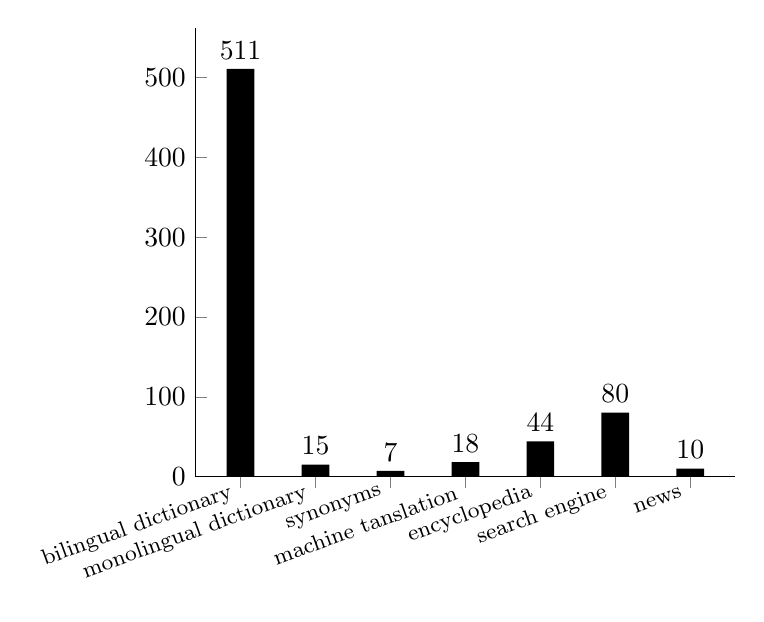
\begin{tikzpicture}
            \begin{axis}[
                    ybar,
                    xtick=data,
                    axis lines*=left,
                    ymin=0,
                    scaled y ticks=false,
%                     colormap/Greys-5,
%                     cycle list/Greys-5,
                    legend pos=north west,
                    reverse legend,
                    nodes near coords,
                    nodes near coords style={color=black},
                    xticklabels={bilingual dictionary,monolingual dictionary,synonyms,machine tanslation,encyclopedia,search engine,news},
                    x tick label style={rotate=20,anchor=east,font=\footnotesize},   
                    legend style={font=\footnotesize},
%                     enlarge x limits={0.1},                
                    ]
                \addplot+[
                     fill=black,draw=none
                    ] coordinates {(0,511) (1,15) (2,7) (3,18) (4,44) (5,80) (6,10)};   
                \legend{}
            \end{axis} 
\end{tikzpicture}
\end{figure}

 


This result concurs with %\label{ref:ZOTEROITEMCSLCITATIONcitationID4ucdoZP2propertiesformattedCitationNord2002plainCitationNord2002dontUpdatetruecitationItemsid18urishttpzoteroorgusers1255332items252Z7TJQurihttpzoteroorgusers1255332items252Z7TJQitemDataid18typebooktitleHilfsmittelbeimbersetzeneineempirischeStudiezumRechercheverhaltenprofessionellerbersetzercollectiontitleFASKPublikationendesFachbereichsAngewandteSprachundKulturwissenschaftderJohannesGutenbergUniversittMainzinGermersheimcollectionnumberBd32publisherLangpublisherplaceFrankfurtamMainNewYorknumberofpages286sourceLibraryofCongressISBNeventplaceFrankfurtamMainNewYorkISBN3631393318callnumberP3065N672002shortTitleHilfsmittelbeimbersetzenauthorfamilyNordgivenBrittaissueddateparts2002schemahttpsgithubcomcitationstylelanguageschemarawmastercslcitationjsonRNDPjB7sALB48}
\citegen[95--96]{Nord2002}
conclusion on the state of the art of translation aids research. The empirical studies showed that bilingual dictionaries are used most often, although critical dictionary research is very sceptical towards them. Although %\label{ref:ZOTEROITEMCSLCITATIONcitationIDf4KhX5ufpropertiesformattedCitationDaemsetal2016plainCitationDaemsetal2016citationItemsid139urishttpzoteroorgusers1255332itemsQ53HQ4XIurihttpzoteroorgusers1255332itemsQ53HQ4XIitemDataid139typechaptertitleTheEffectivenessofConsultingExternalResourcesDuringTranslationandPosteditingofGeneralTextTypescontainertitleNewDirectionsinEmpiricalTranslationProcessResearchpublisherSpringerpublisherplaceHeidelbergNewYorkaopage111133eventplaceHeidelbergNewYorkaoauthorfamilyDaemsgivenJokefamilyCarlgivenMichaelfamilyVandepittegivenSoniafamilyHartsuikergivenRobertfamilyMackengivenLieveeditorfamilyCarlgivenMichaelfamilyBangaloregivenSrinivasfamilySchaeffergivenMoritzissueddateparts2016schemahttpsgithubcomcitationstylelanguageschemarawmastercslcitationjsonRNDDq3DAG3T2h}
\citet[116--117]{DaemsEtAl2016} did not differentiate between monolingual and bilingual dictionaries, the overall results on types of websites used seem to be comparable: The largest group of used aids is by far concordancers and dictionaries (which are represented in monolingual and bilingual dictionaries in this study). Search engines and encyclopedias were the two resources next in line of the aids used most often – although search engines seem to play a more important role for %\label{ref:ZOTEROITEMCSLCITATIONcitationIDLxoWPIzbpropertiesformattedCitationDaemsetal2016plainCitationDaemsetal2016citationItemsid139urishttpzoteroorgusers1255332itemsQ53HQ4XIurihttpzoteroorgusers1255332itemsQ53HQ4XIitemDataid139typechaptertitleTheEffectivenessofConsultingExternalResourcesDuringTranslationandPosteditingofGeneralTextTypescontainertitleNewDirectionsinEmpiricalTranslationProcessResearchpublisherSpringerpublisherplaceHeidelbergNewYorkaopage111133eventplaceHeidelbergNewYorkaoauthorfamilyDaemsgivenJokefamilyCarlgivenMichaelfamilyVandepittegivenSoniafamilyHartsuikergivenRobertfamilyMackengivenLieveeditorfamilyCarlgivenMichaelfamilyBangaloregivenSrinivasfamilySchaeffergivenMoritzissueddateparts2016schemahttpsgithubcomcitationstylelanguageschemarawmastercslcitationjsonRNDhwIMacEGS2}
Daems et al.'s participants than for the participants of this study. News websites were used in both experiments and played a minor role. Interestingly, MT was used by Daems et al.'s participants as a research aid, although the study looked at TfS and PE, while MT was only used in MPE by the participants of this study and never for TfS or PE (see \figref{fig:9:8}).



\begin{figure}
\caption{The use of online aids separated by tasks; left – monolingual post-editing; middle – post-editing; right – human translation}
\label{fig:9:9}
% % \includegraphics[width=\textwidth]{figures/DissertationNitzkeberarbeitet-img23.jpg}
\begin{tikzpicture}[trim axis right,trim axis left]
\pgfplotstableread[col sep=tab]{data/Fig9.9.csv}{\table}
    \pgfplotstablegetcolsof{\table}
    \pgfmathtruncatemacro\numberofcols{\pgfplotsretval-1}
        \begin{axis}[
                    ybar,
                    xtick=data,
                    axis lines*=left,
                    xticklabels from table={\table}{P},
                    bar width=3mm,
                    width=\textwidth,
                    height=5cm,
                    ymin=0,
                    xticklabel style={font=\footnotesize},
                    nodes near coords style={font=\footnotesize},                    
                    enlarge x limits=0.2,
                    colormap/Accent,
                    cycle list/Accent,
                    legend pos=north west,
                    reverse legend,
                    legend style={at={(0.5,-0.25)},anchor=north,font=\footnotesize},
                    legend columns=2,
                    ymax=35,
                    restrict y to domain*=0:40,
                    visualization depends on=rawy\as\rawy, % Save the unclipped values
                        after end axis/.code={ % Draw line indicating break
                            \draw [ultra thick, white, decoration={snake, amplitude=1pt}, decorate] (rel axis cs:0,1.05) -- (rel axis cs:1,1.05);
                         },
                    nodes near coords={%
                            \pgfmathprintnumber{\rawy}% Print unclipped values 
                    },
                    clip=false
                    ]
            \foreach \i in {1,...,\numberofcols} {
                \addplot+[
                    /pgf/number format/read comma as period, fill,draw=none
                    ] table [x index={1},y index={\i},x expr=\coordindex] {\table};
                \pgfplotstablegetcolumnnamebyindex{\i}\of{\table}\to{\colname} % Adding column headers to legend
                \addlegendentryexpanded{\colname}
            }   
            \end{axis}    
\end{tikzpicture}
\end{figure}
 


What becomes obvious at first glance is that bilingual dictionaries are used more often in TfS (82.6\% of all TfS research) than in PE (71.0\%) and finally in MPE (62.0\%) in relation to other consulted resources. As mentioned before, it is very striking that MT engines were only used in the MPE task (11.0\%). The reason is simple: The replays reveal that MT engines were consulted to recreate the source text so that the participants could use the back translation to make more sense of the raw MT output. It is inexplicable why the behaviour between the participants of this study and the study of %\label{ref:ZOTEROITEMCSLCITATIONcitationID9yV3quCapropertiesformattedCitationDaemsetal2016plainCitationDaemsetal2016citationItemsid139urishttpzoteroorgusers1255332itemsQ53HQ4XIurihttpzoteroorgusers1255332itemsQ53HQ4XIitemDataid139typechaptertitleTheEffectivenessofConsultingExternalResourcesDuringTranslationandPosteditingofGeneralTextTypescontainertitleNewDirectionsinEmpiricalTranslationProcessResearchpublisherSpringerpublisherplaceHeidelbergNewYorkaopage111133eventplaceHeidelbergNewYorkaoauthorfamilyDaemsgivenJokefamilyCarlgivenMichaelfamilyVandepittegivenSoniafamilyHartsuikergivenRobertfamilyMackengivenLieveeditorfamilyCarlgivenMichaelfamilyBangaloregivenSrinivasfamilySchaeffergivenMoritzissueddateparts2016schemahttpsgithubcomcitationstylelanguageschemarawmastercslcitationjsonRNDrKBIUTrpAn}
\citet{DaemsEtAl2016} differs so much concerning MT systems as an aid. Maybe the translation training of their participants was more focused on MT systems and hence they acknowledge MT systems as a valuable aid. Or MT systems have a better reputation for their participants than for the participants of this study. This, however, is mere speculation.



The data were tested for independence with \isi{Chi-Square Test}s to find out if different patterns of the websites were used in the respective tasks. All tests turned out to be significant (all three tasks: $\chi^2(12, N=1186)=85.17$, $p<0.0001$; TfS vs. PE: $\chi^2(5, N=522)=18.3$, $p<0.003$; MPE vs. PE: $\chi^2(6, N=346)=28.22$, $p<0.0001$; and TfS vs. MPE: $\chi^2(6, N=502)=51.68$, $p<0.0001$). Hence, the behaviour of the participants varies significantly in the different tasks, although similar patterns can be recognised such the preference for bilingual dictionaries.



Next, the research behaviour between the two groups will be analysed according to the tasks. The use of bilingual dictionaries is the research choice number one, independent of task and status.


\begin{figure}
\caption{Different kinds of websites used for research according to the participant's status (green: professionals; purple: semi-professionals)}
\label{fig:9:10}
% % \includegraphics[width=\textwidth]{figures/DissertationNitzkeberarbeitet-img24.jpg}
\begin{tikzpicture}[trim axis right,trim axis left]
\pgfplotstableread[col sep=tab]{data/Fig9.10.csv}{\table}
    \pgfplotstablegetcolsof{\table}
    \pgfmathtruncatemacro\numberofcols{\pgfplotsretval-1}
        \begin{axis}[
                    ybar,
                    xtick=data,
                    axis lines*=left,
                    xticklabels from table={\table}{P},
                    bar width=4pt,
                    width=\textwidth,
                    height=5cm,
                    ymin=0,
                    xticklabel style={font=\footnotesize},
                    nodes near coords style={font=\footnotesize},
%                     enlarge y limits={upper,value={2}},
                    enlarge x limits=0.1,
                    colormap/Accent,
                    cycle list/Accent,
                    legend pos=north west,
                    reverse legend,
                    legend style={at={(0.5,-0.4)},anchor=north,font=\footnotesize},
                    legend columns=2,
                    ymax=35,
                    restrict y to domain*=0:40,
                    visualization depends on=rawy\as\rawy, % Save the unclipped values
                        after end axis/.code={ % Draw line indicating break
                            \draw [ultra thick, white, decoration={snake, amplitude=1pt}, decorate] (rel axis cs:0,1.05) -- (rel axis cs:1,1.05);
                         },
                    nodes near coords={%
                            \pgfmathprintnumber{\rawy}% Print unclipped values 
                    },
                    clip=false
                    ]
            \foreach \i in {1,...,\numberofcols} {
                \addplot+[
                    /pgf/number format/read comma as period, fill,draw=none
                    ] table [x index={1},y index={\i},x expr=\coordindex] {\table};
                \pgfplotstablegetcolumnnamebyindex{\i}\of{\table}\to{\colname} % Adding column headers to legend
                \addlegendentryexpanded{\colname}
            }
            \end{axis}    
            \node [align=center, text width=3cm, inner sep=0.25cm,font=\footnotesize] at (2, -0.8) {MPE};
            \node [align=center, text width=4cm, inner sep=0.25cm,font=\footnotesize] at (5.6, -0.8) {PE};
            \node [align=center, text width=4cm, inner sep=0.25cm,font=\footnotesize] at (9, -0.8)  {Human Translation};
\end{tikzpicture}
\end{figure}




\figref{fig:9:10} shows that the types of websites used for research differ visibly in MPE and in TfS according to status. Keeping in mind that translation students performed much more research than professionals (see also \tabref{tab:9:8} for total numbers and proportion values), professionals use encyclopedias and search engines more often than students in these two tasks. This is a trend which cannot be detected in PE. The chi-square test confirms this impression – the differences between both groups turn out to be significant in MPE ($\chi^2(6, N=163)=25.61$, $p<0.0003$) and in TfS ($\chi^2(5, N=339)=42.24$, $p<0.0001$). Further, the test did not prove significant for the PE task ($\chi^2(4, N=183)=8.59$, $p=0.0721$). Additionally, it is quite striking that students use bilingual dictionaries far more often as a research tool in TfS than they do in MPE and PE.


\begin{table}
 \small
\begin{tabularx}{\textwidth}{Qrrrrrr}
\lsptoprule
 & \multicolumn{2}{c}{ MPE} & \multicolumn{2}{c}{ PE} & \multicolumn{2}{c}{ HT}\\\cmidrule(lr){2-3}\cmidrule(lr){4-5}\cmidrule(lr){6-7}
 Website type & Prof. & Students & Prof. & Students & Prof. & Students\\
 \midrule 
 \tablevspace 
 Bilingual dictionaries & 40 (0.56) & 61 (0.67) & 29 (0.67) & 101 (0.72) & 79 (0.68) & 201 (0.9)\\
 \tablevspace 
 Monolingual dictionaries & 1 (0.01) & 3 (0.03) & 1 (0.02) & 1 (0.01) & 8 (0.07) & 1 (0.00)\\
 \tablevspace 
 Synonym dictionaries & 0 (0) & 4 (0.04) & 0 (0) & 0 (0) & 0 (0) & 3 (0.01)\\
 \tablevspace 
 MT & 4 (0.06) & 14 (0.15) & 0 (0) & 0 (0) & 0 (0) & 0 (0)\\
 \tablevspace 
 Encyclopedia & 10 (0.14) & 1 (0.01) & 2 (0.05) & 16 (0.11) & 13 (0.11) & 2 (0.01)\\
 \tablevspace 
 Search engine & 13 (0.18) & 8 (0.09) & 8 (0.19) & 21 (0.15) & 16 (0.14) & 14 (0.06)\\
 \tablevspace 
 News & 4 (0.06) & 0 (0) & 3 (0.07) & 1 (0.01) & 0 (0) & 2 (0.01)\\
\lspbottomrule
\end{tabularx}
%%please move \begin{table} just above \begin{tabular
\caption{Count of types of websites used for research according to task and status – Research Times}
\label{tab:9:7}
\end{table}


It is hard to explain, why the research patterns for MPE resemble the patterns of TfS more than the PE patterns concerning the kinds of websites used. Especially if we keep in mind that the analysis so far showed similar patterns for PE and TfS and deviating patterns for MPE.


\newpage 
Moreover, it seems very peculiar that students use bilingual dictionaries by far the most for TfS and encyclopedias most often in PE. While professionals use bilingual dictionaries in the same relation in TfS and PE, the consistent use of bilingual dictionaries in TfS probably indicates a lower proficiency in the students \ili{English} skills. Lexical problems arise in TfS, which are already partly solved by the MT output in the PE tasks. Students seem to consider bilingual dictionaries the most valid tool to overcome lexical problems, while they might encounter other kinds of problems in the PE tasks. The use of encyclopedias, however, indicates semantic research, which may have been useful in MPE, but no reason comes to mind why semantic research might be more important in PE than in TfS. Finally, the number of participants is very low. Hence, this tendency might only have occurred by chance.


\subsection{Time spent on research}
\label{sec:9:2:7}

\begin{quote}
H\textsubscript{6.1}: Participants need more time on research per single word\slash phrase in PE than in TfS. Students need longer to find a translation than professionals if they research.
\end{quote}

 

\begin{figure}[b]
\caption{Mean time per research and task}
\label{fig:9:11}
% % \includegraphics[width=\textwidth]{figures/DissertationNitzkeberarbeitet-img25.jpg}
\begin{tikzpicture}
            \begin{axis}[
                    ybar,
                    xtick=data,
                    axis lines*=left,
                    ymin=0,
                    scaled y ticks=false,
                    colormap/Greys-5,
                    cycle list/Greys-5,
                    legend pos=north west,
                    reverse legend,
                    xticklabels={MPE,PE,TfS},
                    ticklabel style={font=\footnotesize},
                    legend style={font=\footnotesize},
                    width=.5\textwidth,
                    enlarge x limits={0.1},                
                    ]
                \addplot+[
                     fill=black,draw=none
                    ] coordinates {(0,13.42671) (1,12.39145) (2,13.469075)};
                \legend{}                                                                                       
            \end{axis}                                                                                          
\end{tikzpicture}\hspace{10mm}
\begin{tikzpicture}[trim axis right,trim axis left]
        \begin{axis}[
                    ybar,
                    xtick=data,
                    axis lines*=left,
                    ymin=0,
                    scaled y ticks = false,
                    colormap/Greys-5,
                    cycle list/Greys-5,
                    legend pos=south east,
                    reverse legend,
                    xticklabels={MPE,PE,TfS},
                    ticklabel style={font=\footnotesize},
                    legend style={font=\footnotesize,cells={anchor=west}},              
                    width=.5\textwidth,                                           
                    enlarge x limits={0.1},
                    bar width=3mm,
                    legend style={font=\footnotesize},
                    legend columns=-1
                    ]
                \addplot+[
                     fill=Greys-E,draw=none
                    ] coordinates {(0,13.52989) (1,12.51346) (2,14.9938)};
                \addlegendentryexpanded{Professional}                              
                \addplot+[
                     fill=Greys-I,draw=none
                    ] coordinates {(0,13.32353) (1,12.26944) (2,11.94435)}; 
                \addlegendentryexpanded{Student}
            \end{axis}  
\end{tikzpicture}
\end{figure}

 
When we look at productivity and effort, we also have to consider the time translators spent on every research instance. I assume that – if research is conducted – research for one word\slash phrase takes longer in PE than in TfS, because the translator is primed by the MT output and has to overcome this first translation suggestion. At first glance, there appears to be no difference between the time needed for research in all three tasks (see \figref{fig:9:11}). The mean research times per research instance are very similar – MPE: 13.42~s, PE: 12.33~s, TfS: 13.04~s. Further, the \isi{standard deviation} is very high for all three tasks (MPE:~13.89, PE: 8.74~s, TfS: 11.33~s), which shows that there is a lot of variety between the individual subjects, but also between the individual search instances.


When dividing the data by time, both groups need on average a similar amount of time for each research instance in MPE (professionals mean: 13.53~s, sd: 15.78~s; students mean: 13.32~s, sd: 12.12~s) and PE (professionals mean: 12.51~s, sd: 11.36~s, students mean: 12.27~s, sd: 7.62~s). However, the difference is noticeable in TfS (professionals – mean: 14.99~s, sd: 15.33~s, students – mean: 11.94~s, sd: 8.12~s). Also, there is no significant correlation between experience and research time neither for the whole data set, nor for the separate tasks (see \tabref{tab:9:8}).


\begin{table}
\fittable{\begin{tabular}{l *{4}{l@{}S[table-format=-1.5]}}
\lsptoprule
 & \multicolumn{2}{c}{Total } & \multicolumn{2}{c}{MPE } & \multicolumn{2}{c}{PE } & \multicolumn{2}{c}{HT}\\
 \midrule 
 r & r(741) = & -0.0572 & r(186) = & -0.0622 & r(153) = & -0.0589 & r(357) = &-0.051\\
 p &          & 0.1194  &          & 0.3962  &          & 0.4132  &          & 0.3348\\
\lspbottomrule
\end{tabular}}
\caption{Correlation tests between task and experience for research time}
\label{tab:9:8}
\end{table}




The research process takes equally long in all tasks and does not depend on experience. The participants read the website output and then decide whether it is useful or whether they have to consult another aid. However, with many more participants it might be possible to detect significant differences. Hence, the hypothesis could not be confirmed.


\begin{quote}
H\textsubscript{6.2}: Participants spend more time on research in TfS than in PE in the overall session. Students spent more time on research than professionals.
\end{quote}



Next, we want to have a look at how much time the participants spent on average for Internet research according to task, status, and experience. On average, the participants spent 9.03\% (sd:~11.07\%) in MPE, 7.95\% (sd:~5.24\%) in PE, and 10.49\% (sd:~7.08\%) in TfS of the total session duration on Internet research.


\begin{figure}
\caption{Mean Percentage of total session duration spent on Internet research}
\label{fig:9:12}
% % \includegraphics[width=\textwidth]{figures/DissertationNitzkeberarbeitet-img26.jpg}
\begin{tikzpicture}
            \begin{axis}[
                    ybar,
                    xtick=data,
                    axis lines*=left,
                    ymin=0,
                    scaled y ticks=false,
                    colormap/Greys-5,
                    cycle list/Greys-5,
                    legend pos=north west,
                    reverse legend,
                    xticklabels={MPE,PE,TfS},
                    ticklabel style={font=\footnotesize},
                    legend style={font=\footnotesize},
                    width=.5\textwidth,
                    enlarge x limits={0.1},                
                    ]
                \addplot+[
                     fill=black,draw=none
                    ] coordinates {(0,7.98) (1,7.13) (2,10.59)};
                \legend{}                                                                       
            \end{axis}                                                                           
\end{tikzpicture}\hspace{10mm}
\begin{tikzpicture}[trim axis right,trim axis left]
        \begin{axis}[
                    ybar,
                    xtick=data,
                    axis lines*=left,
                    ymin=0,
                    scaled y ticks = false,
                    colormap/Greys-5,
                    cycle list/Greys-5,
                    legend pos=south east,
                    reverse legend,
                    xticklabels={MPE,PE,TfS},
                    ticklabel style={font=\footnotesize},
                    legend style={font=\footnotesize,cells={anchor=west}},              
                    width=.5\textwidth,                                           
                    enlarge x limits={0.1},
                    bar width=3mm,
                    legend style={font=\footnotesize},
                    legend columns=-1
                    ]
                \addplot+[
                     fill=Greys-E,draw=none
                    ] coordinates {(0,8.34) (1,4.43) (2,8.24)};
                \addlegendentryexpanded{Professional}              
                \addplot+[                                     
                     fill=Greys-I,draw=none
                    ] coordinates {(0,7.65) (1,9.37) (2,12.74)}; 
                \addlegendentryexpanded{Student}
            \end{axis}  
\end{tikzpicture}
\end{figure}

 


In total, the least time for research compared to the total session duration is spent during PE, followed by MPE, and most time is spent on human translation as can be seen in \figref{fig:9:12}. Professionals and students spent a similar amount of time on Internet research compared to the total session duration in the MPE task (professionals – mean: 8.34\%, sd: 10.96\%; students – mean: 7.65\%, sd: 11.65\%). However, professionals spent less time on the Internet relative to the total session duration for PE (mean: 4.43\%, sd: 3.28\%) and TfS (mean: 8.24\%, sd: 6.66\%) than the student group (PE – mean: 9.37\%, sd: 5.63\%; TfS – mean: 12.74\%, sd: 6.76).



When we look at the correlation between experience and time related to total session length, there is no statistical significance for MPE ($r_\tau(-1.17)=-0.184$, $p=0.243$) and PE ($r_\tau(-0.96)=-0.151$, $p=0.3349$), but for TfS ($r_\tau(-2.47)=-0.367$, $p=0.01357$). On the other hand, when the statistical test is performed by grouping the participants into students and professionals using a Mann-Whitney-U-test, the test turns out significant for PE ($W=28.5$, $p=0.0409$) and not significant in TfS ($W=44$, $p=0.122$). The test for MPE remains non-significant ($W=64.5$, $p=0.9499$).\footnote{See discussion of the different statistical results in \sectref{sec:9:4}}



Here again, we can see that MPE seems to be equally unfamiliar for students and professionals as they spent an equal percentage of the total session duration on research. While students spent more time on research for PE and most for TfS, professionals spent less time for research in the TfS task and the least for PE. This, again, might have two reasons. First, the professionals may be more proficient in \ili{English} than the student translator, because they have more work experience and second, they might be more confident about lexical choices, both for the choices they make from their own knowledge as well as for the choices from the research suggestions.


\largerpage
The first hypothesis of H\textsubscript{5.2} cannot be confirmed as the participants spent almost equally long on research instances, no matter which task. There seems to be a tendency that professionals need longer for research in general and especially in TfS than students. However, the correlation between experience and time did not become significant. So, the second part of the first hypothesis cannot be confirmed, either. The second hypothesis, on the other hand, can be confirmed. Participants spend more time on research in PE than in TfS and students spent more time on research than professionals.


\subsection{Research according to phases in translation process}
\label{sec:9:2:8}

\begin{quote}
H\textsubscript{7}: Translators research most in the drafting phase in TfS, while they conduct most research in the orientation and revision phase in PE.
\end{quote}



In newer versions of the \isi{TPR database}, three phases are indicated for keylogging and eyetracking data (Version 2.310 was used for this particular analysis) – an orientation, a drafting and a revision phase, which were probably appointed automatically, as well (see discussion below). Here, we assume a macro-level of phases, meaning there is only one \isi{orientation phase} at the beginning, one \isi{drafting phase} and a concluding \isi{revision phase}. Therefore, the research instances were assigned to the single phases (see \tabref{tab:9:9}). Orientation and revision on micro-units that might be indicated by pauses as suggested by %\label{ref:ZOTEROITEMCSLCITATIONcitationIDRaXQLCHYpropertiesformattedCitationJakobsen2002plainCitationJakobsen2002citationItemsid113urishttpzoteroorgusers1255332itemsN4C78J5Furihttpzoteroorgusers1255332itemsN4C78J5FitemDataid113typechaptertitleTranslationdraftingbyprofessionaltranslatorsandbytranslationstudentscontainertitleEmpiricalTranslationStudiesProcessandProductcollectiontitleCopenhagenStudiesinLanguagecollectionnumber27publisherSamfundslitteraturpublisherplaceCopenhagenpage191204eventplaceCopenhagenauthorfamilyJakobsengivenArntLykkeeditorfamilyHansengivenGydeissueddateparts2002schemahttpsgithubcomcitationstylelanguageschemarawmastercslcitationjsonRNDg3HPynVmYv}
\citet{Jakobsen2002} is not taken into consideration in this analysis. I suspect that the participants resort to Internet research on demand in TfS when they want to translate the problematic source text unit, because only few problems are recognised during the orientation phase. Further, research in the revision phase is only necessary to recheck their translation decision. In MPE\slash PE, on the other hand, research is much more distributed among the orientation and revision phase, because the MT output might produce translation suggestions that are not trustworthy, and which have to be approved before and after the drafting phase.


\begin{table}
\begin{tabular}{*{7}{l}}
\lsptoprule
 & \multicolumn{2}{c}{ Orientation} & \multicolumn{2}{c}{ Draft} & \multicolumn{2}{c}{ Revision}\\\cmidrule(lr){2-3}\cmidrule(lr){4-5}\cmidrule(lr){6-7}
& Mean & SD & Mean & SD & Mean & SD\\
 \midrule
 MPE & 0.16 & 0.57 & 0.93 & 1.47 & 0.30 & 0.64\\
 PE & 0.12 & 0.33 & 2.45 & 2.36 & 0.38 & 0.73\\
 TfS & 0.20 & 0.46 & 3.88 & 3.83 & 1.51 & 2.17\\
\lspbottomrule
\end{tabular}
\caption{Mean Research Instances per Translation Phase}
\label{tab:9:9}
\end{table}


As more research took place in TfS than in PE, and least in MPE, the numbers will be compared in total numbers and proportions:


\begin{itemize}
\item MPE: Orientation: 7 (0.12), Drafting: 40 (0.67), Revision: 13 (0.22)
\item PE: Orientation: 5 (0.04), Drafting: 103 (0.83), Revision: 16 (0.13)
\item TfS: Orientation: 8 (0.03), Drafting: 159 (0.69), Revision: 62 (0.27)
\end{itemize}

The most research was done in the drafting phase in all three tasks, followed by the revision phase, and the least research was done in the orientation phase. When we compare the phase distribution of the research instances with the experience of the participants, we find no significant difference for neither the orientation phase ($r_\tau(-1.92)=-0.145$, $p=0.05437$) nor the revision phase ($r_\tau(-0.74)=-0.053$, $p=0.4593$), but instead for the drafting phase ($r_\tau(-2.91)=-0.196$, $p<0.004$). Similar results can be found when testing whether there is a significant difference between the groups (orientation phase {$W=1759.5$, $p=0.06684$, drafting phase $W=1320.5$, $p<0.001$, revision phase $W=1994.5$, $p=0.9173$;} see discussion in \sectref{sec:9:4}). This means that the research behaviour in the orientation and revision phase is very similar, independent of the experience, but the more experienced the translator, the less research (s)he does in the drafting phase. The correlation is very low though.



Unfortunately, we have to assume that the mapping of the phases in the data might have been defective in a few cases. For example, participant 22 translated Text~4 and the orientation phases was only defined as 0.59 minutes, the drafting phase lasted another 0.04 minutes and the rest of the session consisted of revision according to the tables. However, based on common knowledge, we can assume that the drafting phase in a translation session would take longer than two to three seconds. Accordingly, much of the research became part of the revision phase. Hence, the results would have been even clearer if the mapping had been 100\% accurate. As, on the one hand, excluding the obvious mistakes would only have reinforced the result and not shifted it, and on the other hand knowing when to set the limit to exclude data or not would be difficult. Hence, no data points were dismissed.



Conclusively, H\textsubscript{7} cannot be confirmed, because most research is conducted in the drafting phase in all three tasks, although this is done to different degrees.


\subsection{Research ending in no obvious result}
\label{sec:9:2:9}

\begin{quote}
H\textsubscript{8}: Students re-check their translations more often than professionals.
\end{quote}



There were a number of instances in which the research instance did not end in any immediate results, i.~e. research took place, which did not effect the translation product directly, but is part of the translation process. Four categories of these instances, which did not lead directly to a translation result, were found in the data: The Internet was used for \isi{context research} (CR), the word\slash phrase was not translated (\isi{no translation} – NT), the participant read the MT of the machine translated target text (\isi{read back translation} – RBT – only occurred in MPE), and the translator stuck with his\slash her former translation (SFT).

\begin{table}
\begin{tabular}{lrrrrr}
\lsptoprule
 Status & CR & NT & RBT & SFT & Total\\
 \midrule 
 Professional & 10 & 6 & 0 & 30 & 46\\
 Student & 3 & 13 & 1 & 48 & 65\\
 Total & 13 & 19 & 1 & 78 & 111\\
\lspbottomrule
\end{tabular}
\caption{Amount of research instances ending in no (obvious) results}
\label{tab:9:10}
\end{table}





All in all, there were 111 instances in which the participants did some research in the Internet without any direct results (see \tabref{tab:9:10}), which is 14.9\% of all instances. Looking at simple counts, this occurred mostly in student research - professionals: 46, students: 64. However, if it is put in relation to the total instances during which each group conducted research, it occurred more often for professionals (17.2\%, students: 13.4\%). Further, the categories were differently distributed. Most of the times, the non-direct-result research ended in SFT (70.3\%), then NT (17.1\%), CR (11.7\%), and finally RBT (0.01\%). When the status of the participant is taken into consideration, the distribution changes a little. While SFT (professionals: 65.2\%, students: 73.9\%) occurs the most in both groups, NT is more often the result for students (20\%, professionals: 13.0\%) and professionals do more CR (21.7\%, students: 4.6\%). RBT only occurred once in a student translation (1.5\%, professionals: 0\%).


 
\begin{figure}
\caption{Distribution and amount of research instances ending in no (obvious) results according to status (left) and kind of non result (right)}
\label{fig:9:13}
% % \includegraphics[width=\textwidth]{figures/DissertationNitzkeberarbeitet-img27.jpg}
\begin{tikzpicture}[trim axis right,trim axis left]
        \begin{axis}[
                    ybar,
                    xtick=data,
                    axis lines*=left,
                    ymin=0,
                    scaled y ticks = false,
                    colormap/Greys-5,
                    cycle list/Greys-5,
                    legend pos=south east,
                    reverse legend,
                    ticklabel style={font=\footnotesize}, 
                    legend style={at={(0.9,0.4)},anchor=north,font=\footnotesize,cells={anchor=west}},              
                    width=.5\textwidth,                                           
                    enlarge x limits={0.1},
                    bar width=3mm,
                    legend style={font=\footnotesize},
                    xticklabels={},
                    xtick style={draw=none}
                    ]
                \addplot+[
                     fill=Greys-E,draw=none
                    ] coordinates {(0,46)};
                \addlegendentryexpanded{Professional}              
                \addplot+[                                     
                     fill=Greys-I,draw=none
                    ] coordinates {(0,65)}; 
                \addlegendentryexpanded{Student}
            \end{axis}  
\end{tikzpicture}\hspace{10mm}
\begin{tikzpicture}
            \begin{axis}[
                    ybar,
                    xtick=data,
                    axis lines*=left,
                    ymin=0,
                    scaled y ticks=false,
                    colormap/Greys-5,
                    cycle list/Greys-5,
                    legend pos=north west,
                    reverse legend,
                    xticklabels={CR,NT,RBT,SFT},
                    ticklabel style={font=\footnotesize},
%                     legend style={font=\footnotesize},
                    width=.5\textwidth,
                    enlarge x limits={0.1},                
                    ]
                \addplot+[
                     fill=black,draw=none
                    ] coordinates {(0,13) (1,19) (2,1) (3,78)};
%                 \legend{}                                                                       
            \end{axis}                                                                           
\end{tikzpicture}
\end{figure}


\largerpage
Interestingly, over 70\% of the research conducted without any obvious result was caused by the translators' deciding to stick with their former translation or the MT output which can be seen as an indicator of insecurity in their own translation or the MT output. A similar observation was already made by %\label{ref:ZOTEROITEMCSLCITATIONcitationIDERZ0kgeXpropertiesformattedCitationHansPeterKrings1986plainCitationHansPeterKrings1986citationItemsid1709urishttpzoteroorggroups3587itemsX92T2ZTGurihttpzoteroorggroups3587itemsX92T2ZTGitemDataid1709typebooktitleWasindenKpfenvonbersetzernvorgehtEineempirischeUntersuchungzurStrukturdesbersetzungsprozessesanfortgeschrittenenFranzsischlernernpublisherGunterNarrVerlagpublisherplaceTbingeneventplaceTbingennoteZuglBochumUnivDiss198586authorfamilyKringsgivenHansPeterissueddateparts1986schemahttpsgithubcomcitationstylelanguageschemarawmastercslcitationjsonRNDcaTQdkwigX}
\citet[translated by J.~N.]{Krings1986} were he states that “the participants could improve the inferencing solution in 15 cases (39.5\%) by using a dictionary, the solution was confirmed in 20 cases (52.6\%), and in three cases (7.9\%) the solution was impaired by using a dictionary.”\footnote{“In 15 Fällen (39,5\%) konnten die Versuchspersonen das Inferenzierungsergebnis durch die Wörterbuchbenutzung verbessern, in 20 Fällen (52,6\%) wurde das Ergebnis bestätigt, in 3 Fällen (7,9\%) wurde es durch die Wörterbuchbenutzung verschlechtert.”} Although Kring's group of participants (see \sectref{sec:5:3}) is not comparable to the participants of this study, it shows that insecurity with the translation first rendered is a common phenomenon. Similarly translators' insecurity was described by %\label{ref:ZOTEROITEMCSLCITATIONcitationID9B4KPuYVpropertiesformattedCitationPrassl2010plainCitationPrassl2010citationItemsid225urishttpzoteroorgusers1255332itemsNQ5FRI5Purihttpzoteroorgusers1255332itemsNQ5FRI5PitemDataid225typearticlejournaltitleTranslatorsdecisionmakingprocessesinresearchandknowledgeintegrationcontainertitleNewapproachesintranslationprocessresearchpage5782authorfamilyPrasslgivenFriederikeissueddateparts2010schemahttpsgithubcomcitationstylelanguageschemarawmastercslcitationjsonRNDQ5bsJs43lu}
\citet[59--60]{Prassl2010}. She describes that emotions like intuition can make even very convincing possibilities for translation decisions seem unsuitable, which can lead to insecurity towards this possible translation choice. “In translation, we encounter situations in which the subject has already written down a piece of TT [=target text, J.N.] and suddenly stops to go on searching, very often wisely so.” (ibid.: 60)



Further, a non-translation does not necessarily mean that content was omitted, but can also mean that redundancies were avoided, because the content was already delivered in another part of the sentence or another phrase. Finally, content research and reading the back translation can be seen as positive instances of research with no direct result, because the translator familiarises him\slash herself with the text or the context of the text. When both groups are separated we can see the different patterns the groups used (\figref{fig:9:14}).



\begin{figure}
\caption{Types of no-research according to status of the participant}
\label{fig:9:14}
% % \includegraphics[width=\textwidth]{figures/DissertationNitzkeberarbeitet-img28.jpg}
\begin{tikzpicture}
            \begin{axis}[
                    ybar,
                    xtick=data,
                    axis lines*=left,
                    ymin=0,
                    scaled y ticks=false,
                    colormap/Greys-5,
                    cycle list/Greys-5,
                    legend pos=north west,
                    reverse legend,
                    xticklabels={CR,NT,RBT,SFT},
                    ticklabel style={font=\footnotesize},
                    legend style={font=\footnotesize},
                    width=\textwidth,
                    height=5cm,
                    enlarge x limits={0.1},                
                    ]
                \addplot+[
                     fill=Greys-E,draw=none
                    ] coordinates {(0,10) (1,6) (2,0) (3,30)};
                \addlegendentryexpanded{Professional}              
                \addplot+[                                     
                     fill=Greys-I,draw=none
                    ] coordinates {(0,3) (1,13) (2,1) (3,48)};
                \addlegendentryexpanded{Student}                                                                    
            \end{axis}                                                                           
\end{tikzpicture}
\end{figure} 



While both groups predominantly found no result after their research, because they opted for their translation, it happened much more often in the students group than in the group with professional translators. The same applies to non-translations. However, the professionals found no results more often due to context research than students. More context research was done in the MPE task (7 instances), than in PE (5 instances) and only one context research instance could be found in TfS.


\begin{table}
\begin{tabularx}{.8\textwidth}{Xrrrrr}
\lsptoprule
 Task & CR & NT & RBT & SFT & Total\\
 \midrule 
 MPE & 7 & 7 & 1 & 16 & 31\\
 PE & 5 & 3 & 0 & 36 & 44\\
 TfS & 1 & 9 & 0 & 26 & 36\\
 \midrule
 Total & 13 & 19 & 1 & 78 & 111\\
\lspbottomrule
\end{tabularx} 
\caption{Distribution of research instances ending in no (obvious) results according to task}
\label{tab:9:11}
\end{table}


\begin{table}
\begin{tabularx}{.8\textwidth}{Xrrrrrrrrr}
\lsptoprule 
 Task & \multicolumn{2}{c}{ CR} & \multicolumn{2}{c}{ NT} & \multicolumn{2}{c}{ RBT} & \multicolumn{2}{c}{ SFT} & Total\\\cmidrule(lr){2-3}\cmidrule(lr){4-5}\cmidrule(lr){6-7}\cmidrule(lr){8-9}
 Status & S & P & S & P & S & P & S & \multicolumn{1}{c}{ P} & \\
\midrule 
 MPE & 1 & 6 & 6 & 1 & 1 & 0 & 9 & 7 & 31\\
 PE & 1 & 4 & 3 & 0 & 0 & 0 & 29 & 7 & 44\\
 TfS & 1 & 0 & 4 & 5 & 0 & 0 & 10 & 16 & 36\\
 \midrule 
 Total & 3 & 10 & 13 & 6 & 1 & 0 & 48 & 30 & 111\\
\lspbottomrule
\end{tabularx} 
\caption{Distribution of research instances ending in no (obvious) results according to task and status}
\label{tab:9:12}
\end{table}


\tabref{tab:9:11} shows the distribution of no-result research according to task, \tabref{tab:9:12} according to task and status. Interestingly, students chose their initial translation much more often in the PE task than in the TfS task and much more often than professionals in general. This indicates that students are more insecure about the MT output than professionals. Further, professionals conducted more context research in MPE than students, while students left more words\slash phrases untranslated. However, there were too few research instances to call this a pattern.


\subsection{Summary and conclusion – screen recording data}
\label{sec:9:2:10}

Three main reasons for consulting the Internet can be singled out from the previous analysis: The look up of \isi{lexical problems} in bilingual and monolingual dictionaries, the search for more context information (two typical sources are the consultation of search engines and the websites of newspapers), and the generation of the source text with the help of MT. The latter is only used in the MPE task in the study at hand (in contrast to the research behaviour of the participants in %\label{ref:ZOTEROITEMCSLCITATIONcitationIDxG9tI8KEpropertiesformattedCitationDaemsetal2016plainCitationDaemsetal2016citationItemsid139urishttpzoteroorgusers1255332itemsQ53HQ4XIurihttpzoteroorgusers1255332itemsQ53HQ4XIitemDataid139typechaptertitleTheEffectivenessofConsultingExternalResourcesDuringTranslationandPosteditingofGeneralTextTypescontainertitleNewDirectionsinEmpiricalTranslationProcessResearchpublisherSpringerpublisherplaceHeidelbergNewYorkaopage111133eventplaceHeidelbergNewYorkaoauthorfamilyDaemsgivenJokefamilyCarlgivenMichaelfamilyVandepittegivenSoniafamilyHartsuikergivenRobertfamilyMackengivenLieveeditorfamilyCarlgivenMichaelfamilyBangaloregivenSrinivasfamilySchaeffergivenMoritzissueddateparts2016schemahttpsgithubcomcitationstylelanguageschemarawmastercslcitationjsonRNDdznQjLQ1Y6}
\citealt{DaemsEtAl2016} study). There was no evidence in the data that the participants sought any help on syntactic or grammatical problems.


Participants do more research in TfS than in PE and professionals do less research than students both in TfS and PE, confirming H\textsubscript{1}. This shows that fewer lexical problems occur in PE, because some are already solved by the MT output and some \isi{lexical mistranslations} in the MT output can easily be corrected by consulting the target text. Interestingly, professionals research more in MPE than in PE, which indicates that the source text is often necessary to improve the MT output. While simple lexical errors can be remedied easily in PE due to the source text – making the improvement a task, not a problem if the source lexical item is known to the translators – lexical flaws in the MT output can become a problem in MPE. Further, I detected that professionals refer much more to their internal resources in human translation than students do, because they have long spans between two research instances, but not many words are processed. Similar to H\textsubscript{1,} the\textsubscript{} most words per session are looked up in TfS, then PE, as well as MPE; and students look up more words per session than professionals confirming the first part of hypothesis H\textsubscript{2}. Finally, more research instances are necessary per word in MPE than in PE and TfS, because of the missing source text. The difference between PE and TfS is very narrow, hence part two of H\textsubscript{2} was disproved. Experience does not influence how the look up behaviour is performed.



A whole session went by without the help of any online sources most often in MPE, then in PE, and least often in TfS. While professionals did not need the Internet in over 30\% of the sessions in PE and TfS, students did not use it in less than ten percent. Surprisingly, there is no significant difference between PE and TfS, so that H\textsubscript{3} cannot be confirmed. Further, the complexity of a text measured by reading scores does not seem to influence research behaviour (so H\textsubscript{4} cannot be supported). Complexity does not only refer to reading scores and lexical complexity, but also syntactic complexity or length of sentence etc. Hence, further studies need to be carried out to investigate the topic properly.



As the study has shown, the most important research aid for all three tasks were bilingual dictionaries, both for student and professional translators. Further, students use bilingual dictionaries more often than professionals in all three tasks, confirming H\textsubscript{5}. Hence, I consider it unreasonable to proclaim bilingual dictionaries to be useless for translators, as has been put forward so often in theoretical translation studies according to %\label{ref:ZOTEROITEMCSLCITATIONcitationIDtHegj1JYpropertiesformattedCitationNord2002plainCitationNord2002dontUpdatetruecitationItemsid18urishttpzoteroorgusers1255332items252Z7TJQurihttpzoteroorgusers1255332items252Z7TJQitemDataid18typebooktitleHilfsmittelbeimbersetzeneineempirischeStudiezumRechercheverhaltenprofessionellerbersetzercollectiontitleFASKPublikationendesFachbereichsAngewandteSprachundKulturwissenschaftderJohannesGutenbergUniversittMainzinGermersheimcollectionnumberBd32publisherLangpublisherplaceFrankfurtamMainNewYorknumberofpages286sourceLibraryofCongressISBNeventplaceFrankfurtamMainNewYorkISBN3631393318callnumberP3065N672002shortTitleHilfsmittelbeimbersetzenauthorfamilyNordgivenBrittaissueddateparts2002schemahttpsgithubcomcitationstylelanguageschemarawmastercslcitationjsonRNDmYlJ8t75xq}
\citet{Nord2002}. Empirical analyses prove the discrepancy (see also %\label{ref:ZOTEROITEMCSLCITATIONcitationIDRpk5utaSpropertiesformattedCitationDaemsetal2016plainCitationDaemsetal2016citationItemsid139urishttpzoteroorgusers1255332itemsQ53HQ4XIurihttpzoteroorgusers1255332itemsQ53HQ4XIitemDataid139typechaptertitleTheEffectivenessofConsultingExternalResourcesDuringTranslationandPosteditingofGeneralTextTypescontainertitleNewDirectionsinEmpiricalTranslationProcessResearchpublisherSpringerpublisherplaceHeidelbergNewYorkaopage111133eventplaceHeidelbergNewYorkaoauthorfamilyDaemsgivenJokefamilyCarlgivenMichaelfamilyVandepittegivenSoniafamilyHartsuikergivenRobertfamilyMackengivenLieveeditorfamilyCarlgivenMichaelfamilyBangaloregivenSrinivasfamilySchaeffergivenMoritzissueddateparts2016schemahttpsgithubcomcitationstylelanguageschemarawmastercslcitationjsonRND5eLQI7Caw8}
\citealt{DaemsEtAl2016}) – translators are trained to use bilingual dictionaries and trained to use them to combine their \isi{internal and external knowledge}. The research behaviour is statistically different in TfS and MPE between the two groups concerning types of websites used for research, while their was no significant difference for PE.



The time a participant needs for each single research instance is almost the same in all three tasks and is not correlated with experience, although there are some indications that student translators are slightly faster in TfS. However, this did not prove significant. Hence H\textsubscript{6.1} cannot be confirmed. The participants spent most time of the total session on research in TfS, then in MPE, and least in PE. Separated by status, the picture is a little different: Professionals spent most time on research in relation to the total session duration in MPE, then in TfS, and least in PE. Student translators, however, spent the least time in MPE, then PE, and then TfS, confirming H\textsubscript{6.2} which did not include MPE. However, the relative time is approximately equal for both groups in MPE, which again shows that professionals are much more confident in PE and TfS as they do not do research as randomly as student translators.



Most research took place in the \isi{drafting phase} in all three tasks, which disproves hypothesis H\textsubscript{7}. Finally, there were instances when the participants researched a word\slash phrase, but did not transfer this new knowledge into a target text unit immediately. These instances can be grouped as context research, no translation of the source unit, reading the back translation of the MT output, and choosing the initial translation. Rechecking and opting for the own translation or MT output occurred most often, which indicates insecure behaviour (the risk of a mistranslation is averted). Accordingly, this occurred most often for student participants, which supports hypothesis H\textsubscript{8}. Context research was conducted most often by professionals and no translation of the source unit occurs most in student translations.


\largerpage
Two of the arguments \citet[92]{Nord2002} summarized from other empirical studies were analysed in the study at hand as well. First, that less experienced translators tend to use bilingual dictionaries, while professionals use other aids. It is true that in the study at hand professionals used bilingual dictionaries less often than students, and used monolingual dictionaries, encyclopaedias, and search engines more often in TfS, but this does not apply for PE. Professionals use less of all sources (except news items, which are hardly used anyway) in PE than students. The second argument that professionals do more research on one problem\slash source text unit cannot be confirmed. There was no statistically significant correlation between experience and research instances per word\slash problem.



The research patterns seem very similar for all participants in MPE, independent of their experience as translators. This shows that patterns between PE and TfS are different and also differ according to experience; translation experience influences the PE behaviour, while it has no influence on MPE behaviour. As was already mentioned in the analysis, it is assumed that MPE cannot be connected to the translation task, because strategies and behavioural patterns acquired in TfS cannot be transferred. Compared to the TfS task, the MT output solves problems in the PE task. If the MT output is not acceptable, a look at the source text unit helps the translator to either find an acceptable translation, which can be categorised as a task, or (s)he has to research to find a fitting target text item. However, it can be assumed that the translator would have needed to conduct research for this item in the TfS task, too. However, if the MT output is misleading in the MPE task, a new problem arises which may not have been a problem in the TfS task, because the translator cannot check the source text. Hence, misleading MT output creates new problems only in MPE, but not in PE.


\section[Lexical problem solving: Eyetracking data on most researched words/phrases]{Lexical problem solving: Eyetracking data on most researched words/phrases\sectionmark{Eyetracking data on most researched words/phrases}}\sectionmark{Eyetracking data on most researched words/phrases}
\label{sec:9:3}
\largerpage

This chapter analyses the \isi{eyetracking data} of the most researched words\slash phrases in the six texts. The aim is to investigate whether there is a significant difference between certain eyetracking parameters when words\slash phrases were looked up in the Internet compared to when they were not. It is assumed that when a word\slash phrase needs investigation, the translator lacks some vital information on how to paraphrase the instance in the \isi{target language} or, in other words, how to solve the translation problem. Therefore, more mental effort is needed and more \isi{gaze time} is allocated.



The \isi{CRITT-TPR database} (see \sectref{sec:7:2}) contains tables with keylogging and eyetracking data for each translator and task %\label{ref:ZOTEROITEMCSLCITATIONcitationIDZTDIpzoQpropertiesformattedCitationCarlandSchaeffer2013plainCitationCarlandSchaeffer2013citationItemsid144urishttpzoteroorgusers1255332itemsP4KVCC89urihttpzoteroorgusers1255332itemsP4KVCC89itemDataid144typearticlejournaltitleTheCRITTTranslationProcessResearchDatabaseV14URLhttpbridgecbsdkresourcestprdbTPRDB14pdfauthorfamilyCarlgivenMichaelfamilySchaeffergivenMoritzJissueddateparts2013accesseddateparts2014610schemahttpsgithubcomcitationstylelanguageschemarawmastercslcitationjsonRNDCnd7XxJw6y}
(\citealt{CarlSchaeffer2013}). To compare the data, three parameters were chosen, one concerned with production time (\textit{Dur}) and two with gaze data (\textit{GazeS} and \textit{GazeT}):


\begin{description}
\item[\isi{Dur}] Duration of unit \isi{production time} […]
\item[\isi{GazeS}] Total \isi{gaze time} on source text unit […]
\item[\isi{GazeT}] Total \isi{gaze time} on target text unit […] (ibid.: 22)
\end{description}


\textit{Dur}, \textit{GazeS}, and \textit{GazeT} include all instances in which the target word\slash phrase was produced or the source\slash target word\slash phrases was looked at. Therefore, these parameters can be used to compare technical effort (i.e. production time) and indications of mental effort (i.e. \isi{gaze time} on source and target text) of the particular unit in the overall session. It is important to investigate the whole translation session because the word\slash phrase may not have been considered problematic in the first encounter. It is also not possible to imply that the word\slash phrase became unproblematic after the research instance or the (first) production of the target word\slash phrase. The following hypotheses are proposed for the keylogging and eyetracking data:


\begin{itemize}
\item H\textsubscript{1}: Longer production times and more gaze time can be found for a word\slash phrase when it has been researched in an online aid than when no research was conducted.



H\textsubscript{01}: Production time and gaze data are independent of conducted research.



\item H\textsubscript{2}: Longer production times and more gaze time is needed for TfS compared to PE.



H\textsubscript{02}: Production time and gaze data are independent of the task.



\item H\textsubscript{3}: Further, student translators need longer production times and more gaze than professional translators or, phrased differently, less experienced translators need longer production times and more gaze than more experienced translators.



H\textsubscript{03}: Production time and gaze data are independent of status\slash experience.
 
\end{itemize}



First, all words\slash phrases were filtered that had been looked up in the Internet at least four times to make sure that the word\slash phrase is considered problematic by at least some participants and, hence, worth investigating and that the number of instances is enough to conduct first tests for significance. In the second step, troublesome words\slash phrases were excluded from the list. The following reasons were taken into account:


\begin{itemize}
\item Words\slash phrases that concluded the heading or the text were excluded. When the eyetracking data were assigned, some gaze points were mapped incorrectly. This error occurs particularly often at the end of the headline, because all gaze that occurred in the rest of the empty line was mapped on the last word of the line; and the end of the text, because all gaze that occurred on the rest of the empty window was mapped on the last word of the text.
\item Words\slash phrases that appear more than once in the source text were excluded, because it is impossible to narrow down the problematic instance or whether or not all appearances were equally problematic, etc.
\item Some words\slash phrases were only used for content research, usually proper nouns. Therefore, the word\slash phrase itself was not problematic lexically, but was used to find more information on the topic. For example, participant P17 entered “Stephen Spielberg Olympic Beijing” into a search engine and read a news article about it afterwards.
\end{itemize}

After excluding the research instances that were not interesting for the following analysis, a total of 27 words\slash phrases can be analysed (see \tabref{tab:9:13} and Appendix~II \tabref{tab:B:1}). These include six phrases, two two-item words (i.e. “below-inflation” and “pull out”) and 19 words. All single words were content words, in particular nouns, adjectives, and verbs.


\begin{table}
\begin{tabularx}{\textwidth}{lXXXXXX}
\lsptoprule
 & Text 1 & Text 2 & Text 3 & Text 4 & Text 5 & Text 6\\
 \midrule 
 No. Words/Phrases & 1 & 3 & 10 & 8 & 2 & 3\\
\lspbottomrule
\end{tabularx} 
\caption{Number of Analysed Words distributed per Text}
\label{tab:9:13}
\end{table}


When phrases were looked up, the gaze data were collected for the whole phrase and not only for the words that were actually looked up. For example, in the dependent sub-clause “\textit{which includes one minister charged with crimes against humanity by the International Criminal Court in The Hague}” some translators researched \textit{Criminal Court}, \textit{International Criminal Court}, \textit{International Criminal Court in The Hague}, etc. Hence, the production time and gaze data of the whole phrase \textit{the International Criminal Court in The Hague} was taken into consideration, even if only \textit{Criminal Court} was looked up, so that the different research instances can be compared, no matter how the translator decided to gather information on the phrase.



This chapter summarizes and discusses the results and provides examples from the actual data. In Appendix~\ref{sec:Appendix:B}, all words\slash phrases used for analysis are listed as well as the corresponding mean and the standard variation (which is in most cases very high again; see the discussion in \sectref{sec:9:3:1}. Further, tests for statistical significance were conducted via non-directed t-tests for normal distribution or Mann-Whitney-U-tests for not normally distributed data, and correlations with experience coefficient were calculated (see \sectref{sec:9:3:2}). As the data points were so few and the main focus of the study at hand is on the difference between PE and TfS, not all analyses were performed for MPE as well. However, a more detailed discussion on the participants research behaviour in the MPE task can be found in %\label{ref:ZOTEROITEMCSLCITATIONcitationID5LT8Rc9ipropertiesformattedCitationNitzke2016monobplainCitationNitzke2016monobcitationItemsid183urishttpzoteroorgusers1255332itemsUPJZPQ8Rurihttpzoteroorgusers1255332itemsUPJZPQ8RitemDataid183typechaptertitleMonolingualposteditingAnexploratorystudyonresearchbehaviourandtargettextqualitycontainertitleEyetrackingandAppliedLinguisticspublisherLanguageSciencePresspublisherplaceBerlinpage83108eventplaceBerlinauthorfamilyNitzkegivenJeaneditorfamilyHansenSchirragivenSilviafamilyGruzcagivenSamborissueddateparts2016schemahttpsgithubcomcitationstylelanguageschemarawmastercslcitationjsonRNDTVnYGcHTBE}
\citet{Nitzke2016mono}.


\subsection{Mean values of eyetracking data}
\label{sec:9:3:1}

In most cases, the mean value for all three parameters (\textit{Dur}, \textit{GazeS}, \textit{GazeT}) is higher for research instances than for \isi{no-research instances} (find exact values in Appendix~\ref{sec:Appendix:B}, \tabref{tab:B:2}). This was expected because researching a lexical item on the Internet indicates effort. However, the mean values were higher for the following words\slash phrases for one or more parameter when they were not looked up on the Internet:


\begin{itemize}
\item One parameter higher in no-research instances:


\begin{itemize}
\item \textit{Dur} – pull out, compromise, bureaucrats
\item \textit{GazeS} – embarrass
\item \textit{GazeT} – associate, bureaucrats, full-time leader, artisan
\end{itemize}
\item Two or three parameters higher in no-research instances: 


\begin{itemize}
\item  \textit{Dur}, \textit{GazeS} and \textit{GazeT –} incentives 
\end{itemize}
\end{itemize}

Altogether, 78 mean value pairs were compared (26 words $*$ 3 parameters) – in only 10 instances, the mean value was higher for no-research instances than for research instances (12.8\%). The following paragraphs will discuss some possible explanations as to why the mean values may have been higher. However, as presented in the next chapter, none of these differences are significant. Therefore, it is possible that these instances occurred by chance and we also cannot eliminate the possibility of technical problems or defective gaze mapping.



Longer production times (\textit{Dur}) in no-research instances may have been produced by a wide array of lexical choices that were activated in the participants' minds, while the Internet research may have accelerated the problem solving process. Instead of using the internal resources and pondering about which lexical item to choose, the problem was resolved quicker via Internet research. As a side note, if no Internet research was conducted, it does not necessarily mean that the \isi{translation unit} was not problematic for the participant (if it was problematic, it would explain the high \textit{Dur} time), but we do not have a distinct indicator. Two of the words mentioned above that required longer production times are verbs (\textit{compromise} and \textit{pull out}), which often present a lot of translation choices and need to be adapted to the grammatical and syntactic structures of the sentence. \textit{Compromise} may require additional effort, because it can be both noun and verb. However, this should be a minor effect given the syntactic position in the sentence. The MT output can be considered partly acceptable for both verbs (in both cases parts of the full lexical or grammatical structure are missing), which may have caused longer production times as well. Further, \textit{compromise} has a (more or less) false friend in \ili{German}: \textit{kompromittieren} - “damage one's or someone else's reputation through a statement or a manner; to compromise sb./sth.”\footnote{“durch eine Äußerung oder ein Verhalten jemandes, dem eigenen Ansehen schaden; bloßstellen“} (duden.de\footnote{\url{http://www.duden.de/rechtschreibung/kompromittieren}, last accessed 24\textsuperscript{th} April 2015}). Although \textit{kompromittieren} is one of the meanings of \textit{compromise}, it is not appropriate in the context. Similarly, the word \textit{bureaucrats} has a cognate – words with similar form but different meaning – in \ili{German}, which may have caused higher production times, due to uncertain decision making (the MT system translated the word with the \ili{German} cognate version).



The longer \isi{gaze time} on the source text (GazeS) for \textit{embarrass} might be explained by the syntactically highly complex sentence it is set in. In general, high gaze times on the source text could imply on a lexical level that the word\slash phrase is unknown to the translator, that the word\slash phrase can be categorised as low frequent, that the word\slash phrase is ambiguous, and\slash or that the word\slash phrase is used in an unusual context or in a context it is hardly used in.



Long \isi{gaze time} on the target text (GazeT) might indicate insecurity with the (machine) translation of the source item. The MT output for the above mentioned words varies a lot: the MT output for \textit{associate} is not acceptable, partly acceptable for \textit{full-time leader}, and acceptable for \textit{artisan}. Further, all three words are not embedded in informative context (\textit{associate} is used to explain the Latin origin of another word; \textit{full-time leader} and \textit{artisan} are parts of a list), which may cause more insecurity with the MT output or the translation choice.



\textit{Incentives} (a low frequency word) seemed to be a very problematic term as it required a lot of effort when it was not researched. All three parameters were on average higher when the word was not looked up on the Internet. The MT system did not translate the word so the MT output was of no help in the PE task. It could even be considered a burden – a hurdle between source and target text – because the untranslated word has to first be deleted in the target text.



All in all, the discussion of the mean values showed that no research does not mean that the participants did not struggle to come up with a good solution. However, the results strongly indicate that research causes more processing and \isi{production effort} because the mean values are in most instances higher for research instances than for no-research instances. It would be interesting to test, whether there is a certain threshold at which the eyetracking data would indicate at which point translators fall back on their inner resources.


\subsection{Statistical tests for eyetracking data}
\label{sec:9:3:2}

First, the data for all 27 words\slash phrases were compared as a whole data set. The first point of interest was whether there is a significant difference between research instances and no-research instances in those words. The tests turned out to be significant for all three parameters: \textit{Dur}: $W=21670.5$, $p<0.0001$; \textit{GazeS}: $W=27137$, $p<0.0001$; \textit{GazeT}: $W=32385$, $p=0.001$. As the tests were not directed, the mean values were taken into consideration and they showed that all three parameters are higher for research instances than for no-research instances. In other words, the production time of researched words as well as the \isi{gaze duration} on the source and target text is in general significantly higher when the participants research the word.



In a next step, we look at different sub-tests. First, it was tested whether there is still a significant difference between research and no-research, when only TfS and PE are taken into consideration together (Test 1) and for the each task individually (Test 2-4). Then, whether there is a significant difference between TfS and PE as well as between professionals and students independent of research behaviour (Test 5). The next tests investigated whether there is a difference in the research\slash no-research data for professionals and then for students combining the tasks (Test 6 and 7). The following three tests (Test 8, 9, and 10) considered whether there is a difference between the status of the participants in TfS, PE, and MPE. The last \isi{Mann-Whitney-U-tests} focused on task and status (Test 11 and 12). In a final step, correlations were calculated for parameters and experience, experience and task, experience and research\slash no-research instance.



To summarise the results, nine of thirteen Mann-Whitney-U-tests (69.2\%) became significant for the parameter \textit{\isi{Dur},} and one of six (16.7\%) correlations. 11 of 13 Mann-Whitney-U-tests (84.6\%) became significant for \isi{total fixation duration} on the source text (\textit{GazeS}) and two of six (33.3\%) correlations. The tests for \textit{GazeT} did not turn significant that often: three of thirteen Mann-Whitney-U-tests (23.1\%) became significant and none of the correlation tests. \textit{Dur} is not significant for status in general and, in particular, status considering the single tasks. This means that the production times of rather problematic words do not depend on the status of the participant. This is also mirrored in the correlation with experience. The production time and the experience coefficient only correlate when the words\slash phrases are produced without doing any research and the correlation is very weak, too. Gaze duration on the source text (\textit{GazeS}) always became significant, except when only MPE was taken into consideration. The test for MPE needs to be excluded though, because there was only one window in the MPE task. Nonetheless, gaze was mapped on the source and the target text, which is a technical error. The correlations were only significant when experience was correlated with the overall \textit{GazeS} and experience and PE. Both tests showed a (very) very small negative correlation. This means the more experienced a participant is the less (s)he looks at the source text item. However, the correlations are so small that the difference is hardly recognisable. \textit{GazeT} only became significant when compared between TfS and PE, meaning that there is a significant difference between TfS and PE concerning gaze on the target text; and when the student data were compared for when they conducted research and when they did not.



The next chapter provides detailed insights on the single words\slash phrases. Five tests for significance were conducted for every word\slash phrase and for every parameter that was taken into consideration in the last chapter, which results in twelve tests for significance per word\slash phrase:


\begin{itemize}
\item First, it was tested whether there is a \textbf{significant} \textbf{difference} \textbf{between} \textbf{research} \textbf{instances} \textbf{and} \textbf{no-research} \textbf{instances}, independent of the tasks. First, all three tasks will be considered and then only PE and TfS in a second test.
\item Then, a test was conducted on whether there is a \textbf{significant} \textbf{difference} \textbf{between} \textbf{PE} \textbf{and} \textbf{TfS}, independent of research behaviour.
\item The last two tests calculated whether \textbf{the} \textbf{difference} \textbf{between} \textbf{research} \textbf{and} \textbf{no-research} \textbf{was} \textbf{significant} \textbf{in} \textbf{TfS} \textbf{and} \textbf{PE}, respectively.
\end{itemize}

\tabref{tab:9:14} summarises how often the tests proved significance for all 28 analysed words and phrases. In these calculations, most tests for significance did not turn into a significant result. One explanation is the low number of instances (n) that can be analysed – especially in the last two tests – and therefore, the chances that the difference occurred by accident are too high. The data, for example, only presented one research instance for “halt” in the PE data which was than compared to six no-research instances. When testing significant differences between research and no-research for the single tasks, some tests could not be conducted, because the word\slash phrase was not researched in the task. However, some tests became significant and in the following, these significant differences will be discussed. As the tests were undirected, the mean values were used to identify which values were significantly higher\slash lower. 

\begin{table}
% % \small
% % \begin{tabularx}{\textwidth}{lrrrrr}
% % \lsptoprule
% %  & \multicolumn{5}{c}{p-value <~0.05}\\
% %  Parameter & research yes/no (all) & research yes/no  (PE and TfS) & different tasks  (PE vs. TfS) & research yes/no for TfS &  { research yes/no for PE}\\
% %  \midrule 
% %  \isi{Dur}   & 10 & 6 & 7 & 1 & 0\\
% %  GazeS & 5 & 2 & 8 & 1 & 0\\
% %  GazeT & 4 & 3 & 4 & 1 & 0\\
% % \lspbottomrule
% % \end{tabularx}
\begin{tabular}{lrrr}
\lsptoprule
& \multicolumn{3}{c}{Parameter}\\\cmidrule(lr){2-4}
& \isi{Dur} & GazeS & GazeT\\\midrule
research yes/no (all) & 10 & 5 & 4       \\
research yes/no  (PE and TfS) & 6 & 2 & 3\\
different tasks  (PE vs. TfS) & 7 & 8 & 4\\
research yes/no for TfS &  1 & 1 & 1 \\
research yes/no for PE& 0 & 0 & 0    \\
   \lspbottomrule
\end{tabular}
\caption{Number of tests with $p<0.05$\label{tab:9:14}}
\end{table}


As the tests were not directed, it was verified whether the parameters were significantly higher or lower when research was conducted compared to when no research was conducted or according to task. In all cases, the parameters turned out to be significantly higher when research was conducted. The test between TfS and PE, however, did not compare research\slash no research but the tasks. Interestingly, the parameters were significantly lower for PE in all cases.



The data suggest that more effort was necessary when the participants decided to research words\slash phrases compared to when they translated the same words\slash phrases without the help of any Internet resource, although only 52 of the 405\footnote{3 parameters $*$ 5 tests (research yes\slash no; research yes\slash no in TfS only; research yes\slash no in PE only) $*$ 28 words\slash phrases – 15 tests that could not be conducted due to missing data (e.\ g. when none of the participant researched the word\slash phrase in the \isi{post-editing} task).} tests (12.5\%) became significant, which might mainly be caused by the low n-values as mentioned above. This argument is strengthened by the fact that, when all data from all three tasks were used for testing significance, 19 tests turned out to be significant, while when the research instance in one single task was tested none (for PE) and three (for TfS) proved significant.



The tests that compared TfS and PE and were significant and in favour of PE, meaning that PE took less processing and \isi{production effort} than TfS. In total, 19 of the 78\footnote{3 parameters $*$ 26 words\slash phrases} tests (24\%) turned out to be significant. Here again, a bigger data collection might have led to more obvious results. Nonetheless, the results are in favour of MT as an aid on the lexical level for the PE process. Accordingly, the hurdle between source text and target text might sometimes be overcome by the MT output and sometimes not. However, the data do not suggest that MT creates new hurdle.



Again, the parameter \textit{GazeT} was the least productive of the three parameters. However, the difference is not that obvious as it was when all words were compared. Twelve tests for \textit{GazeT} became significant, while “only” 16 tests for \textit{GazeS} became significant, which is only 33.3\% more. Eleven tests became significant for \textit{GazeS} in the overall data, while only three for \textit{GazeT} became significant. Two reasons could explain these differences between single words\slash phrases and overall data. First, the lower n-value might cause far fewer tests for \textit{GazeS} to turn significant. Second, there could be some words\slash phrases with very extreme data that influence the overall results rather than the single words\slash phrases. However, most tests for single words\slash phrases that became significant have p-values between 0.01 and 0.05, which does not implicate extreme values. Conclusively, this implies that problem solving is handled rather on a source text level than on a target text level.


\subsection{Further analysis – Misleading machine translation}
\label{sec:9:3:3}

In contrast to what might have been expected, even if the participants had decided that the MT output was unacceptable for the target text, \isi{processing and production effort} does not increase significantly in the PE task. Although some mean values of the parameters are higher in the PE task than in TfS (see \sectref{sec:9:3:1}), these few instances are more the exception than the rule. Hence, we will look at the influence of \isi{misleading MT}. The purpose of \isi{post-editing} MT output is to produce a target text more efficiently. Therefore, MT should reduce lexical problems and conclusively reduce research effort. However, practice shows that MT systems occasionally choose the wrong lexical entry for the context, which results in misleading or wrong translations in the MT output. These have to be corrected by the post-editor and hence a productivity gain cannot be detected.



Two of the most researched words\slash phrases were looked up more often in the PE task than in the TfS task (\textit{compromise} and \textit{incentives} – both were already discussed in \sectref{sec:9:3:1} on mean values). The increased research effort might be caused by the PE task, which in a way restricts the participants. The translators have to use the MT output as a translation frame, which makes them work less freely. Hence, the target text representation might be primed by the MT output and cause less associations in the brain. However, this increased research effort is the exception not the rule – in our examples it only occurred in less than 8\% of the analysed words. Usually more research is performed in TfS. Looking at it the other way around, this low figure rather speaks in favour of MT than against it. Especially, when we look at the other words\slash phrases that were predominantly researched in TfS. \textit{Insistence} and \textit{flaring up again} were researched only in TfS and research was about equally distributed between TfS and PE in only a few examples like \textit{associate} or \textit{serve}. Hence, MT rather decreased the research necessity in the overall sessions, which supports the assumption mentioned earlier that MT helps to deconstruct hurdles rather than to erect new ones.


\subsection{Comparing most researched words to least-/no-research words}
\label{sec:9:3:4}

In this chapter, we will compare words\slash phrases that were researched most often with comparable (or as comparable as possible) words\slash phrases that did not require research by most participants. Three words\slash phrases were picked for analysis from the 27 most researched, for which comparable words\slash phrases could be found in the relatively small text corpus provided by the six texts.



First, we will compare the phrase “the International Criminal Court in The Hague” (1) which was looked up eight times and “China's backing for Sudan's policy in Darfur”(2)\footnote{To avoid typing the entire phrases every time they need to be referred to, they will be referred to as Phrase (1) and Phrase (2) in the following.}, where parts of the phrases were looked up in six sessions, mostly for context research. In this respect, Phrase (2) was not considered a whole phrase by the participants but as single units, while Phrase (1) was considered one unit. Both phrases consist of seven words and a similar amount of characters (45 and 44, respectively, including spaces). Further, the MT output is not very error prone for both phrases, although the MT for Phrase (2) is missing one definite article\footnote{(1) MT: „den Internationalen Strafgerichtshof in Den Haag"  (2) MT: „Chinas Unterstützung für Sudan-Politik in Darfur"}. Both phrases contain proper nouns, Phrase (1) an institutional name and a location name, and Phrase (2) three location names. There are \ili{German} equivalents for the institutional and the location name of Phrase (1), whereas all location names in Phrase (2) can be retained. However, Phrase (2) is grammatically more complex. Another advantage of comparing these phrases is that they occurred in the same text. Hence, the participants translated the phrases within the same task and individual differences could be ruled out.



Next, the word \textit{rattle} (looked up eleven times) will be compared to \textit{adapt} (no research instances occurred) and \textit{disliked} (looked up twice in the human translation tasks). \textit{Adapt} and \textit{disliked} were chosen for comparison, because they are both verbs, even though \textit{disliked} is used in the simple past and is therefore grammatically more complex; they also have comparable frequencies. The TPR-DB indicates frequencies as the log10 probabilities according to the \isi{\textit{British National Corpus}} (cf. %\label{ref:ZOTEROITEMCSLCITATIONcitationIDonwur0kjpropertiesformattedCitationCarlandSchaeffer2013plainCitationCarlandSchaeffer2013citationItemsid144urishttpzoteroorgusers1255332itemsP4KVCC89urihttpzoteroorgusers1255332itemsP4KVCC89itemDataid144typearticlejournaltitleTheCRITTTranslationProcessResearchDatabaseV14URLhttpbridgecbsdkresourcestprdbTPRDB14pdfauthorfamilyCarlgivenMichaelfamilySchaeffergivenMoritzJissueddateparts2013accesseddateparts2014610schemahttpsgithubcomcitationstylelanguageschemarawmastercslcitationjsonRNDtRspSIs78e}
\citealt{CarlSchaeffer2013}: 15), which are for \textit{rattle} \textminus5.5360, for \textit{adapt} \textminus5.0924, and for \textit{dislike} \textminus5.3152. \textit{Dislike}, however, is a special case because it is followed by another verb (\textit{working}) and hence is often realised as an adverb, like in the MT output 'nicht gern […] arbeiten' ('not willingly […] work'). Nonetheless, it was considered for comparison.



Finally, we will look at three adjectives with similar frequencies: \textit{vulnerable} – looked up eight times, frequency: \textminus4.7104; \textit{extra} (as it occurred in text 2) – not researched, frequency: \textminus4.1181; \textit{extensive} – researched once, frequency: \textminus4.4829.



I compared the parameter \textit{Dur}, \textit{GazeS}, and \textit{GazeT} for research in TfS and PE, research in TfS, research in PE, according to task (TfS vs. PE), high research words\slash phrase against low research words\slash phrase (general, for TfS and PE, for TfS, for PE, for TfS and research, for TfS and no research, for PE and research, and for PE and no research).



In total, 19 of 108\footnote{3 word categories $*$ 3 parameters $*$12 test conditions} tests (17.6\%) turned out significant. The most promising test was comparing PE and TfS, which turned out significant in seven out of nine instances (77.8\%). As the tests were undirected, the mean values were evaluated and it was always the PE sessions that showed less keylogging activity or \isi{eye movement}. The parameter \textit{Dur} is the most meaningful in the verbs chapter and turned out significant seven out of twelve times, while it was hardly significant for adjectives and phrases. Surprisingly, \textit{Gaze S} and \textit{GazeT} turned out significant equally often for all word\slash phrase-categories, namely five times (which is still not much), but no tendencies for one word\slash phrase-category can be detected.



In a final test series, a high frequency verb and a high frequency adjective were compared to the highly researched verb and adjective as the latter were low frequency words (\textit{vulnerable} vs. \textit{new} and \textit{rattle} vs. \textit{have}). The tests were conducted both with the original data and normalised to the number of characters. The most promising parameter was again \textit{Dur}. Interestingly, the results of the tests were not as extreme as expected as only three of the 36 normalised tests turned significant for both verbs and adjectives.


\subsection{Status and experience}
\label{sec:9:3:5}

In this chapter, we will analyse how experience (considering both the \isi{participants' status} and \isi{experience vector}) influences the parameter comparing highly researched words and low researched words as introduced in the previous chapter. Again, one aim of this analysis is to compare which measurement for experience might be more helpful for statistical analysis.



When we compare professionals and students, statistically significant differences cannot be observed often. Differences only appear in \textit{GazeS}, if at all, for all tasks or only for TfS or PE. \textit{Dur} becomes significantly different in the verbs chapter for students and professionals considering research and no-research, no matter whether we compare low-frequency verbs or low- and high-frequency verbs. The students group shows a significant difference in \textit{Dur} and \textit{GazeS}, when we compare low- and high-frequency adjectives, which is not observable for professionals. When we look at the differences in tasks, all parameters are higher in TfS for students and professionals. Almost the same tests became significant for both groups, except for phrases regarding the \isi{gaze behaviour}. In the latter case, professionals needed significantly longer to read source and target text units in the TfS task, while there was no difference for student translators. Finally, when we compare high-research and low-research words\slash phrases, the difference is significant much more often for students (six times) than for professionals (once). Interestingly, the only parameter that became significant for professionals – \textit{Dur} for adjectives – became significantly higher for low-research words, while all significant instances for students were higher for high-research words.



The \isi{experience factor} was a not very informative value in this analysis. Three of 18 tests (16.6\%) became significant for the overall data. When we tested most researched words against low\slash no-research words, only one of 168 tests (0.6\%) became significant. The test that became significant described the correlation between experience and \isi{gaze duration} on the source text in the PE task when comparing high-research and low-research phrases. Again, we can only speculate that the number of data points is too small to turn out significant correlations or simply that no connection exists between experience and keylogging behaviour as well as \isi{eye movement}.



In one final attempt to find statistical significant relations, a \isi{linear mixed model}\footnote{Using the packages "effects", "lmerTest" %\label{ref:ZOTEROITEMCSLCITATIONcitationIDL1NjhXOppropertiesformattedCitationKuznetsovaBrockhoffandChristensen2015plainCitationKuznetsovaBrockhoffandChristensen2015noteIndex124citationItemsid4071urishttpzoteroorgusers1255332itemsRYF7BS7Murihttpzoteroorgusers1255332itemsRYF7BS7MitemDataid4071typearticlejournaltitlePackagelmerTestcontainertitleRpackageversionvolume2issue0authorfamilyKuznetsovagivenAlexandrafamilyBrockhoffgivenPerBruunfamilyChristensengivenRuneHauboBojesenissueddateparts2015schemahttpsgithubcomcitationstylelanguageschemarawmastercslcitationjsonRND4sLVRbykPa}
\citep{KuznetsovaEtAl2015}, and "lme4" %\label{ref:ZOTEROITEMCSLCITATIONcitationIDVZ7Huqc5propertiesformattedCitationBatesetal2014plainCitationBatesetal2014noteIndex124citationItemsid4072urishttpzoteroorgusers1255332items6Q2BVS4Vurihttpzoteroorgusers1255332items6Q2BVS4VitemDataid4072typearticlejournaltitlelme4LinearmixedeffectsmodelsusingEigenandS4containertitleRpackageversionpage123volume1issue7authorfamilyBatesgivenDouglasfamilyMaechlergivenMartinfamilyBolkergivenBenfamilyWalkergivenStevenliteralothersissueddateparts2014schemahttpsgithubcomcitationstylelanguageschemarawmastercslcitationjsonRNDsUV52Jq4xt}
\citep{BatesEtAl2014}.} was created for the most researched words. The individual participants and the different texts were set as random effects in the calculation. Task and research were included in the model. The data for MPE was excluded for the GazeS and GazeT models, because the mapping was arbitrary. There was an attempt to integrate status and\slash or experience into the model, but they did not influence the model significantly, and therefore were excluded. First, let us look at \textit{Dur}. \textit{Dur} is significantly different between TfS and MPE ($t=\pm2.28$, $p=0.0228$), but not between TfS and PE ($t=\pm1.61$, $p=0.107$) or PE and MPE ($t=\pm0.77$, $p=0.4426$). Further, it is significantly higher when research was conducted ($t=4.61$, $p<0.0001$). Total \isi{fixation duration} on the source text (\textit{GazeS}) is higher for TfS ($t=4.82$, $p<0.0001$) and when research was conducted ($t=3.05$, $p=0.0025$). Finally the \isi{total fixation duration} on the target text is higher for TfS as well ($t=1.98$, $p=0.0486$), but no significant difference can be found when research was conducted and when not ($t=1.60$, $p=0.1108$).


\subsection{Summary and conclusion – Keylogging and eyetracking data}
\label{sec:9:3:6}

The most promising process parameter appears to be \textit{Dur}, which seems quite reasonable, because the parameter describes production duration. Hence, the participants needed longer to produce these problematic words. This can either mean that many changes occurred during the session or that the participants literally needed more time to produce the word, because they might have thought about whether the translation decision is correct or suitable, or might have considered other options.



The eyetracking parameters were not as conclusive, but \textit{GazeS} is more promising than \textit{GazeT}. Higher \textit{GazeS} times indicate problematic words\slash phrases. However, a problematic word\slash phrase does not necessarily trigger a higher \isi{reading time}. The problem might not be caused by the source item itself as the translator knows what it means, but by transfer to the target text. Hence, this problematic situation might not be reflected in the \isi{reading time} of the source text item itself, but in the whole surrounding text area, because the translator needs to grasp the context and transfer the problematic item to the context. On the other hand, it is reasonably safe to assume that \isi{reading time} of the target text item does not reflect on problematic translation units, although we have to consider the lack of data points. Finally, a lot of the processing probably occurs during the research instance itself. The translator looks for examples for a solution in a bilingual dictionary. While (s)he does this, (s)he has the context in mind and integrates the research effort into the context. Hence, a reasonable solution might already be created during the research process, which is obviously not recognisable in the reading data of source and target text item. 



Interestingly, the differences between PE and TfS were very often significant when similar words\slash phrases that caused different research behaviour were compared, except for \textit{GazeT} in two cases. This indicates that the MT output is helpful for both words\slash phrases that were researched very often and that were not\slash hardly researched.



When comparing data for single tasks and\slash or only for research\slash no research instances, hardly any tests turned out significant. However, when the mean values are compared, a difference is often recognisable. The reason for the insignificant tests is either that there are no significant difference and\slash or that we do not have enough data points to compare the data. Some tests were not possible at all, because there were, for example, no research instances in the PE task. Conclusively, a larger data set would be necessary to perform meaningful calculations.



In summary, when we look at the overall data set, the hypothesis can be confirmed. Words\slash phrases that were researched often required longer production times and longer gazes on the source text unit. Research does not seem to have an influence on the \isi{gaze duration} on the target text. Hence, more mental effort is necessary, when research is necessary. Further, there is a tendency that text units take longer to produce and are gazed at longer in the source text for TfS. Finally, student translators seem to need longer to produce the text unit and gaze longer at the source text, while no effect could be measured on the target text \isi{reading time}. This, however, was not confirmed in the \isi{linear mixed model}, in which no significant difference could be determined between students and professionals nor does the experience coefficient have a significant influence. Hence, \isi{problem solving behaviour} seems to be indicated by text production time and the \isi{total gaze time} on the source text, but not on the target text.


\section{Overall conclusions and final remarks}
\label{sec:9:4}

The analyses of screen recording as well as eyetracking and keylogging show that sometimes different research patters can be observed both between PE and TfS as well as between students and professionals, while other results are equal between all participants and tasks. Participants did more research in the TfS task than in the PE task. Similarly, students researched more than professionals. Amount of research and experience correlate significantly for TfS and PE. Interestingly, participants decided not to use Internet research as often in PE as in TfS; professionals more often than students, although the test did not prove significant. The correlation of experience and not using Internet research, however, turned significant. When all participants are taken into consideration, the complexity levels of the texts seem to influence the amount of research, but this result might be accidental, because the distribution is different when the participants are separated into groups of professionals and students. Bilingual dictionaries are used most often for research by both groups and in all tasks. The research instances were about equally long, independent of status of the participant and task. The relation between research time and total session duration is almost equal between professionals and students in the MPE task, while it is higher for students than for professionals in PE and TfS. Testing for significance with a \isi{Mann-Whitney-U-test} and correlations presented contradictory results (see discussion below). Most research takes place in the drafting phase and, in most cases, translators choose their first translations if the research instance does not result in a direct target text decision. Students rechecked their translation choice or the MT output much more often than the professionals, which indicates insecurity.



In 87.2\% of cases, the mean values of the eyetracking and keylogging parameters were higher for research instances than for \isi{no-research instances}. When the parameters were tested for significance for the single words\slash phrases, they were not as productive, which is probably caused mainly by the low n-numbers. This argument is strengthened when we look at the overall data set. The tests for significance all resulted in p far below 0.05 when comparing research instances and no research instances, and also by the \isi{linear mixed model}. When single words\slash phrases are examined, the most reliable parameter is \textit{Dur}. Hence, long production times might indicate problematic words. The gaze parameters are not that productive. This might have two reasons: First, the problem might become visible in the reading times of the whole phrase around the problematic word\slash phrase, because the translator processes the context simultaneously; and second, a lot of processing might already occur during research, which is then not identifiable in the gaze data. When testing between two tasks, the tests that became significant were in favour of PE, meaning PE required less effort. Bad quality MT output usually does not increase the writing and reading effort, but it becomes equal to the effort of TfS instead. Hence, MT output solves some translation problems in PE, some are not solved, but no new problems are created either. In MPE, however, new problems are sometimes created because the translator cannot refer to the source text.



The analyses show that translation experience seems to have an influence on PE, because the patterns between students and professionals and the correlations between research behaviour and \isi{experience factor} often suggest differences. However, this result could not be confirmed by the linear mixed model. A larger data set might be helpful to reinvestigate the issue. There were no implications that translation experience influences the MPE task. The task was probably new to all participants meaning they could not apply their usual strategies due to the missing source text.



A high \isi{standard deviation} could be observed in screen-recording, keylogging and eyetracking data. This points to high individual differences in all data. There might be a tendency, towards what is perceived as a translation problem and therefore leads to higher production times and gaze data. Furthermore, less experienced participants might demonstrate different behavioural patterns than more experienced translators. Nonetheless, what is problematic for the individual varies a lot according to their internal knowledge – a parameter which could not be measured in this study.

In general, the \isi{experience vector} was very helpful for the screen-recording observations as it often revealed significant differences. However, the parameter was less productive for keylogging and eyetracking data, which might be caused by the data sparseness. Another interesting aspect that was discussed in \sectref{sec:9:2:6} is that statistical tests turned significant for different tasks, depending on whether they were grouped according to status (professional vs. students) or correlated with experience. The example in \sectref{sec:9:2:6} considered the time spent on research in relation to the total session duration. The test turned out to be significant for PE when the required time was grouped according to status, but not when correlated with experience. Further, the opposite applies when TfS is tested: no significance when comparing groups, but a significant correlation between time and experience. That the tests turned out differently depending on the chosen test is more the exception than the rule. However, I assume that testing the correlation with the \isi{experience factor} is a more valid test than testing with the groups, because the \isi{experience factor} takes the individual differences into account more than grouping the participants according to status. As discussed in \sectref{sec:8:1}, both groups are very homogeneous and more details of personal experience would be desirable. However, as was shown in this chapter on research behaviour, it is still very useful to group the participants into professionals and students, on the one hand for visualisation reasons, and to arrive at a valid impression of the data distribution on the other. In another example, the results were comparable: In \sectref{sec:9:2:8}, we analysed the distribution of research instances on phases, which was analysed according to the experience of the participants. The results were for the orientation phase: $r_\tau(-1.92)=-0.145$, $p=0.05437$, the drafting phase: $r_\tau(-2.91)= -0.196$, $p<0.004$, and the revision phase: $r_\tau(-0.74)=-0.053$, $p=0.4593$, while the results according to status for the orientation phase are: $W=1759.5$, $p=0.06684$, the drafting phase $W=1320.5$, $p<0.001$, and the revision phase $W=1994.5$, $p=0.9173$. These results are very similar and point in the same direction. In the following chapters, I will further investigate whether grouping according to status or experience coefficient is more informative.
